\newif\ifanswers
%\answerstrue % comment out to hide answers
% hack from https://tex.stackexchange.com/questions/33576/conditional-typesetting-build

\documentclass[aspectratio=169
  , xcolor={svgnames}
  , hyperref={ colorlinks,citecolor=DeepPink4
             , linkcolor=DarkRed,urlcolor=DarkBlue}
  , russian
  ]{beamer}
\usetheme{CambridgeUS}
\beamertemplatenavigationsymbolsempty % remove navigation bar
\setbeamertemplate{headline}{}

\usefonttheme{professionalfonts}
\makeatletter
\@ifclassloaded{beamer}{
  % get rid of header navigation bar
  \setbeamertemplate{headline}{}
  % get rid of bottom navigation symbols
  \setbeamertemplate{navigation symbols}{}
  % get rid of footer
  %\setbeamertemplate{footline}{}
}
{}
\makeatother
%%%%%%%%%%%%%%%%%%%%%%%%%%%%%%%%%%%%%%%%%%%%%
\usepackage{fontawesome}
% \newfontfamily{\FA}{Font Awesome 5 Free} % some glyphs missing
\expandafter\def\csname faicon@facebook\endcsname{{\FA\symbol{"F09A}}}
\def\faQuestionSign{{\FA\symbol{"F059}}}
\def\faQuestion{{\FA\symbol{"F128}}}
\def\faExclamation{{\FA\symbol{"F12A}}}
\def\faUploadAlt{{\FA\symbol{"F093}}}
\def\faLemon{{\FA\symbol{"F094}}}
\def\faPhone{{\FA\symbol{"F095}}}
\def\faCheckEmpty{{\FA\symbol{"F096}}}
\def\faBookmarkEmpty{{\FA\symbol{"F097}}}

\newcommand{\faGood}{\textcolor{ForestGreen}{\faThumbsUp}}
\newcommand{\faBad}{\textcolor{red}{\faThumbsODown}}
\newcommand{\faWrong}{\textcolor{red}{\faTimes}}
\newcommand{\faMaybe}{\textcolor{blue}{\faQuestion}}
\newcommand{\faCheckGreen}{\textcolor{ForestGreen}{\faCheck}}
%%%%%%%%%%%%%%%%%%%%%%%%%%%%%%%%%%%%%%%%%%%%%

\usepackage{fontspec}
\usepackage{xunicode}
\usepackage{xltxtra}
\usepackage{xecyr}
\usepackage{hyperref}

\setmainfont[
 Ligatures=TeX,
 Extension=.otf,
 BoldFont=cmunbx,
 ItalicFont=cmunti,
 BoldItalicFont=cmunbi,
% Scale = 1.1
]{cmunrm}
\setsansfont[
 Ligatures=TeX,
 Extension=.otf,
 BoldFont=cmunsx,
 ItalicFont=cmunsi,
%  Scale = 1.2
]{cmunss}
%\setmainfont[Mapping=tex-text]{DejaVu Serif}
%\setsansfont[Mapping=tex-text]{DejaVu Sans}
%\setmonofont{Fira Code}[Contextuals=AlternateOff]
\setmonofont{Fira Code}[Contextuals=Alternate,Scale=0.9]
\newfontfamily{\myfiracode}[Scale=1.5,Contextuals=Alternate]{Fira Code}
%\setmonofont[Scale=0.9,BoldFont={Inconsolata Bold}]{Inconsolata}

\usepackage{polyglossia}
\setmainlanguage{russian}
\setotherlanguage{english}


%\newfontfamily\dejaVuSansMono{DejaVu Sans Mono}
% https://github.com/vjpr/monaco-bold/raw/master/MonacoB/MonacoB.otf
%\newfontfamily\monacoB{MonacoB}
%%%%%%%%%%%%%%%%%%%%%%%%%%%%%%%%%%%%%%%%%%%%%%%5
\usepackage{soul} % for \st that strikes through
\usepackage[normalem]{ulem} % \sout

\usepackage{stmaryrd}
\newcommand{\sem}[1]{\ensuremath{\llbracket #1\rrbracket}}


\usepackage{listings}
%\lstdefinestyle{style1}{
%  language=haskell,
%  numbers=left,
%  stepnumber=1,
%  numbersep=10pt,
%  tabsize=4,
%  showspaces=false,
%  showstringspaces=false
%}
%\lstdefinestyle{hsstyle1}
%{ language=haskell
%%          , basicstyle=\monacoB
%         , deletekeywords={Int,Float,String,List,Void}
%         , breaklines=true
%         , columns=fullflexible
%         , commentstyle=\color{ForestGreen}
%         , escapeinside=§§
%         , escapebegin=\begin{russian}\commentfont
%         , escapeend=\end{russian}
%         , commentstyle=\color{ForestGreen}
%         , escapeinside=§§
%         , escapebegin=\begin{russian}\color{ForestGreen}
%         , escapeend=\end{russian}
%         , mathescape=true
%%          , backgroundcolor = \color{MyBackground}
%}
%
%\newcommand{\inline}[1]{\lstinline{haskell}{#1}}
%\def\hsinline{\mintinline{haskell}}
%\def\inline{\hsinline}
%
%\lstnewenvironment{hslisting} {
%    \lstset { style={hsstyle1} }
%  }
%  {}
%  
%%%%%%%%%%%%%%%%%%%%%%%%%%%%%%%%%%%%%%%%%%%%%%%%%%%%%%%%%%%  
%%\setmainfont[
%% Ligatures=TeX,
%% Extension=.otf,
%% BoldFont=cmunbx,
%% ItalicFont=cmunti,
%% BoldItalicFont=cmunbi,
%%]{cmunrm}
%%% С засечками (для заголовков)
%%\setsansfont[
%% Ligatures=TeX,
%% Extension=.otf,
%% BoldFont=cmunsx,
%% ItalicFont=cmunsi,
%%]{cmunss}
%% \setmonofont[Scale=0.6]{Monaco}
%
%\usefonttheme{professionalfonts}
%\usepackage{times}
\usepackage{tikz}
\usetikzlibrary{cd}
\usepackage{tikz-cd}
\usepackage{caption}
\usepackage{subcaption}

%\renewtheorem{definition}{برهان}[chapter]
%%\DeclareMathOperator{->}{\rightarrow}
%\newcommand\iso{\ensuremath{\cong}}
%\usepackage{verbatim}
%\usepackage{graphicx}
%\usetikzlibrary{arrows,shapes}

%\usepackage{amsmath}
%\usepackage{amsfonts}
\usepackage{scalerel}
\DeclareMathOperator*{\myvee}{\scalerel*{\vee}{\sum}}
\DeclareMathOperator*{\mywedge}{\scalerel*{\wedge}{\sum}}

%
%\usepackage{tabulary}
%
%% sudo aptget install ttf-mscorefonts-installer
%%\setmainfont{Times New Roman}
%%\setsansfont[Mapping=tex-text]{DejaVu Sans}
%
%%\setmonofont[Scale=1.0,
%%    BoldFont=lmmonolt10-bold.otf,
%%    ItalicFont=lmmono10-italic.otf,
%%    BoldItalicFont=lmmonoproplt10-boldoblique.otf
%%]{lmmono9-regular.otf}
%
\usepackage[cache=true]{minted}
\usemintedstyle{perldoc}

\def\hsinline{\mintinline{haskell}}
\def\mlinline{\mintinline{ocaml}}
% color options
\definecolor{YellowGreen} {HTML}{B5C28C}
\definecolor{ForestGreen} {HTML}{009B55}
\definecolor{MyBackground}{HTML}{F0EDAA}



\institute{матмех СПбГУ}

\addtobeamertemplate{title page}{}{
  \begin{center}{\tiny Дата сборки: \today}\end{center}
}

\usepackage{tabulary}
\usepackage{verbatim}
% \usepackage{tabularx}  % for 'tabularx' environment
% \usepackage{ragged2e} % for \Centering macro
% \newcolumntype{C}{>{\Centering\arraybackslash}X}m
% sudo aptget install ttf-mscorefonts-installer
\defaultfontfeatures{Ligatures={TeX}}
\setmainfont{CMU Serif Roman}
\setsansfont{CMU Sans Serif}
\setmonofont{CMU Typewriter Text} % cyrillic issues

%\setmonofont[Scale=1.0,
%    BoldFont=lmmonolt10-bold.otf,
%    ItalicFont=lmmono10-italic.otf,
%    BoldItalicFont=lmmonoproplt10-boldoblique.otf
%]{lmmono9-regular.otf}

\newcommand{\term}[2]{\textit{#1} (#2)}

\usepackage[cache=true]{minted}
\usepackage{amsthm}

\newtheorem{remark}{\textbf{Замечание}}[section]
\newtheorem{hint}{\textbf{Указание разработчикам}}[section]

\newtheoremstyle{exerciseStyle1}
{}                % Space above
{}                % Space below
{}                % Theorem body font % (default is "\upshape")
{}                % Indent amount
{\bfseries}       % Theorem head font % (default is \mdseries)
{.}               % Punctuation after theorem head % default: no punctuation
{ }               % Space after theorem head
{}                % Theorem head spec
\theoremstyle{exerciseStyle1}
\newtheorem{exercise}{\textbf{Упражнение}}[section]


\deftranslation[to=russian]{Theorem}{Теорема}
\deftranslation[to=russian]{theorem}{теорема}

\usepackage{tikz}
\usetikzlibrary{trees}
\usepackage{subcaption}

%%%%%%%%%%%%%%%%%%
\makeatletter
\newenvironment{tabminted}{%
  \let\FV@ListVSpace\relax  
  \minted
}{%
  \endminted
  \unskip   
  \aftergroup\@tabmintedend
}
\newcommand*{\tabminted@finalstrut}[1]{%
  \ifdim\prevdepth>0pt
    \ifdim\dp#1>\prevdepth
      \vskip\dimexpr(\dp#1)-\prevdepth\relax
    \fi
  \else
    \vskip\dimexpr(\dp#1)\relax
  \fi
}
\newcommand*{\@tabmintedend}{%
  \let\@finalstrut\tabminted@finalstrut
}
\renewcommand{\cite}[1]{}
\makeatother

%\tikzset{every picture/.style={/utils/exec={\rmfamily}}}

%%%%%%%%%%%%%%%%%%%%%5
\title[]{Распределение регистров и решение головоломок}
\subtitle{Register Allocation by Puzzle Solving}
\author{Косарев Дмитрий }

\institute{матмех СПбГУ}

\date{18 ноября 2019}
%\date{\today}

\AtBeginSection[]
{
  \begin{frame}<beamer>%[allowframebreaks]
    \frametitle{Оглавление}
    \tableofcontents
      [currentsection
      ,currentsubsection
%      ,sectionstyle=show/hide
%      ,  subsectionstyle=show/shaded 
      ]
  \end{frame}
}

\newcommand{\verbatimfont}[1]{\def\verbatim@font{#1}}
\setcounter{tocdepth}{1}  % part,chapters,sections 
\newcommand\chap[1]{
%  \chapter*{#1}
  \addcontentsline{toc}{chapter}{#1}
}

\usepackage{verbatimbox}

\begin{document}
\maketitle

% For every picture that defines or uses external nodes, you'll have to
% apply the 'remember picture' style. To avoid some typing, we'll apply
% the style to all pictures.
\tikzstyle{every picture}+=[remember picture] 

% By default all math in TikZ nodes are set in inline mode. Change this to
% displaystyle so that we don't get small fractions.
\everymath{\displaystyle}

% Uncomment these lines for an automatically generated outline.
\begin{frame}{Оглавление}
  \tableofcontents[]
\end{frame}

\section{Задача распределения регистров}

\begin{frame}{Задача распределения регистров (register allocation)}
\begin{itemize}
  \item Назначение физических локаций переменным в программе
    \begin{itemize}
      \item регистры быстрые, но их мало
      \item памяти много, но она медленная
    \end{itemize}
  \item Ограничение: переменные, которые \emph{живы одновременно}, должны быть назначены в разные регистры
  \item Если регистров не хватает, то некоторые переменные должны храниться в памяти
\end{itemize}
\end{frame}

\section{Особенности, осложняющие задачу}

\begin{frame}[fragile]{Распределение регистров: что происходит?}
\begin{minipage}{.48\textwidth}
Исходная программа:
\begin{verbatim}
MyVar1  = 2
MyVar2  = 40
MyVar3  = 0
MyVar3 += MyVar1
MyVar3 += MyVar2
print(MyVar3)
\end{verbatim}
\end{minipage}
\begin{minipage}{.48\textwidth}
\begin{figure}
\centering
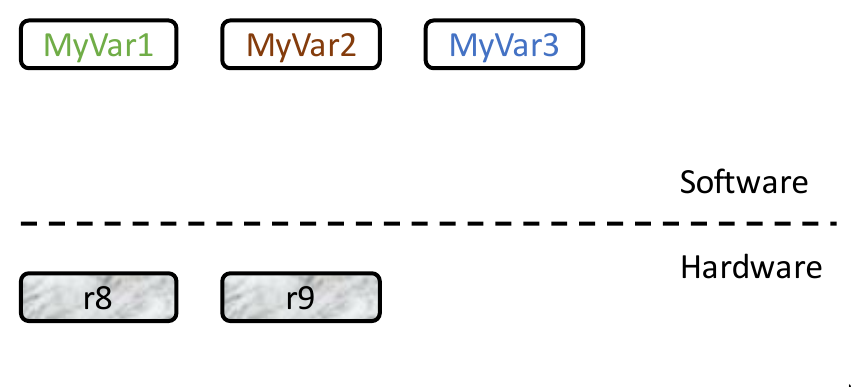
\includegraphics[width=1.\linewidth]{figures/regalloc-demo1}
\end{figure}
\vspace{1cm}
Результат:
\begin{verbatim}
MyVar1  -> stack 
MyVar2  -> r8
MyVar3  -> r9
\end{verbatim}
\end{minipage}

\end{frame}

\begin{frame}[fragile]{}
\begin{minipage}{.48\textwidth}
Исходная программа:
\begin{verbatim}
MyVar1  = 2
MyVar2  = 40
MyVar3  = 0
MyVar3 += MyVar1
MyVar3 += MyVar2
print(MyVar3)
\end{verbatim}
\end{minipage}
\begin{minipage}{.48\textwidth}
\begin{figure}
\centering
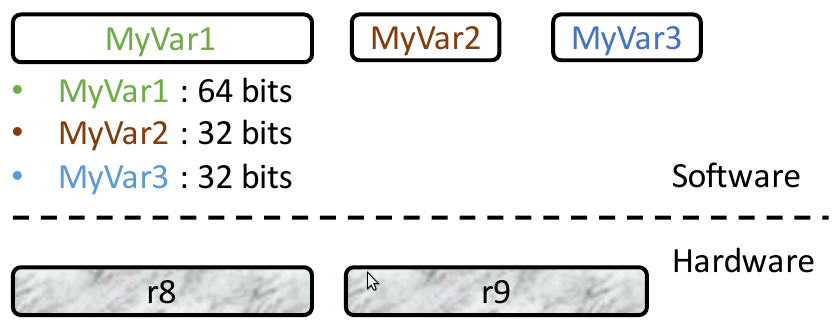
\includegraphics[width=1\linewidth]{figures/regalloc-demo2}
\end{figure}
\vspace{1cm}
Иерархия регистров (aliasing):
\begin{itemize}
\item  r8 может хранить одно 64-битное число или два 32-битных
\item  r9 может хранить 64-битное число
\end{itemize}
\end{minipage}
\end{frame}


\begin{frame}[fragile]{Нерегулярные архитектуры. Pre-coloring}
\begin{minipage}{.48\textwidth}
Вызов функций (PowerPC):
\begin{minted}[escapeinside=??]{text}
a := 10;
b := 2;
?\textcolor{teal}{R0}? := a;
?\textcolor{teal}{R1}? := b;
call(?\textcolor{teal}{R0}?, ?\textcolor{teal}{R1}?);
\end{minted}
\end{minipage}
\begin{minipage}{.48\textwidth}
Деление (x86)
\begin{minted}[escapeinside=??]{text}
a := 10;
b := 2;
?\textcolor{teal}{AX}? := a;
(?\textcolor{teal}{AL}?,?\textcolor{teal}{AH}?) := DIV ?\textcolor{teal}{AX}?, b;
d := ?\textcolor{teal}{AL}?; // частное
r := ?\textcolor{teal}{AH}?; // остаток
\end{minted}
\end{minipage}
\vspace{1em}

Некоторые переменные должны быть связаны с конкретными регистрами из-за соглашений о вызовах, деления и т.п.
\end{frame}


\begin{frame}[fragile]{Нерегулярные архитектуры. Иерархия регситров(aliasing)}
\begin{minipage}{.4\textwidth}
Вложенные регистры могут использоваться как независимо, так и в комбинации с другими\\

Встречается в архитектурах: x86, Sun SPARC, MIPS у чисел плавающей точкой, и т.д.
\end{minipage}
\begin{minipage}{.58\textwidth}

\begin{figure}[h]
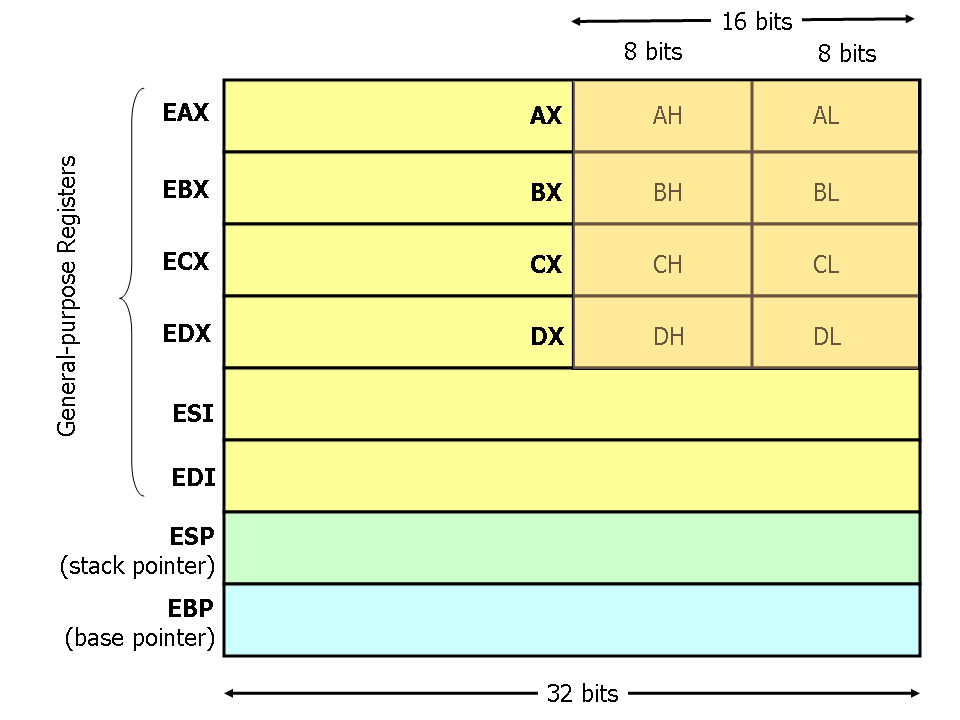
\includegraphics[scale=.35]{figures/x86-registers.png}
\caption{Пример: иерархия регистров у Pentium}
\end{figure}
\end{minipage}
\end{frame}

\section{Терминология}

\begin{frame}{Терминология (1/3). Spilling \& coalescing}
\emph{Spilling}\\
Если регистров не хватает для всех переменных, то некоторые должны храниться в памяти.
Обращение к этим переменным \textbf{неэффективно}\vspace{1cm}

Если области использования переменных \emph{не пересекаются} и они \emph{связаны инструкцией копирования} $v_1=v_2$, то их следует хранить в одном регистре, и это называется \emph{coalesing (объединение)}.
\end{frame}



\begin{frame}{Терминология (2/3). Период жизни переменной}
\noindent{
\begin{minipage}{.5\textwidth}
\begin{figure}[h]
  

\tikzset{every picture/.style={line width=0.75pt}} 
%set default line width to 0.75pt        

\begin{tikzpicture}[x=0.75pt,y=0.75pt,yscale=-1,xscale=1]
%uncomment if require: 
%\path (0,300); %set diagram left start at 0, and has height of 300

\draw [line width=1mm]  (168.57,24.88) -- (168.81,100.02) ;
\draw [line width=1mm]  (196.5,58) -- (196.74,133.14) ;
\draw [line width=1mm]  (166.5,200) -- (166.26,240) ;
\draw [line width=1mm]  (216.5,97.5) -- (216.74,172.64) ;
\draw [line width=1mm]  (243.5,134.86) -- (243.74,210) ;
\draw [line width=1mm]  (263.5,164.86) -- (263.74,240) ;

% Text Node
\draw (77,133) node  [align=left] {{\tt 1) \ \ \ \ \ a := 1}\\\\{\tt 2) \ \ \ \ \ b := 2}\\\\{\tt 3) \ \ \ \ \ c := a}\\\\{\tt 4) \ \ \ \ \ d := b}\\\\{\tt 5) \ \ \ \ \ e := c}\\\\{\tt 6) \ \ \ \ \ a := d}\\\\{\tt 7) \ \ ret a + e}};
% Text Node
\draw (168.57,24.88) node  [align=left] {{\fontfamily{pcr}\selectfont a}\\};
% Text Node
\draw (196.5,58) node  [align=left] {b\\};
% Text Node
\draw (166.5,200) node  [align=left] {{\fontfamily{pcr}\selectfont a}\\};
% Text Node
\draw (216.5,97.5) node  [align=left] {c\\};
% Text Node
\draw (243.5,134.86) node  [align=left] {d\\};
% Text Node
\draw (263.5,164.86) node  [align=left] {e\\};
\end{tikzpicture}
\par
\end{figure}
\end{minipage}}
\begin{minipage}{.48\textwidth}
\begin{itemize}
\item Переменная \emph{живая}, если она может быть использована в будущем
\item \emph{Период жизни (live range)} переменной -- это коллекция точек программы, где она жива.
\end{itemize}
\end{minipage}
\end{frame}

\begin{frame}[fragile]{Распределение регистров  и графы. Пример (1/3)}
\noindent{
\begin{minipage}{.5\textwidth}
\begin{figure}[h]
  

\tikzset{every picture/.style={line width=0.75pt}} 
%set default line width to 0.75pt        

\begin{tikzpicture}[x=0.75pt,y=0.75pt,yscale=-1,xscale=1]
%uncomment if require: 
%\path (0,300); %set diagram left start at 0, and has height of 300

\draw [line width=1mm]  (168.57,24.88) -- (168.81,100.02) ;
\draw [line width=1mm]  (196.5,58) -- (196.74,133.14) ;
\draw [line width=1mm]  (166.5,200) -- (166.26,240) ;
\draw [line width=1mm]  (216.5,97.5) -- (216.74,172.64) ;
\draw [line width=1mm]  (243.5,134.86) -- (243.74,210) ;
\draw [line width=1mm]  (263.5,164.86) -- (263.74,240) ;

% Text Node
\draw (77,133) node  [align=left] {{\tt 1) \ \ \ \ \ a := 1}\\\\{\tt 2) \ \ \ \ \ b := 2}\\\\{\tt 3) \ \ \ \ \ c := a}\\\\{\tt 4) \ \ \ \ \ d := b}\\\\{\tt 5) \ \ \ \ \ e := c}\\\\{\tt 6) \ \ \ \ \ a := d}\\\\{\tt 7) \ \ ret a + e}};
% Text Node
\draw (168.57,24.88) node  [align=left] {{\fontfamily{pcr}\selectfont a}\\};
% Text Node
\draw (196.5,58) node  [align=left] {b\\};
% Text Node
\draw (166.5,200) node  [align=left] {{\fontfamily{pcr}\selectfont a}\\};
% Text Node
\draw (216.5,97.5) node  [align=left] {c\\};
% Text Node
\draw (243.5,134.86) node  [align=left] {d\\};
% Text Node
\draw (263.5,164.86) node  [align=left] {e\\};
\end{tikzpicture}
\par
\end{figure}
\end{minipage}}
\begin{minipage}{.48\textwidth}
Вопросы:
\begin{itemize}
\item Сколько нужно регистров для этой программы?
\item Существует ли универсальный алгоритм?
\item P или NP?
\end{itemize}

\end{minipage}
\end{frame}


\begin{frame}[fragile]{Распределение регистров и графы. Пример (2/3)}
\noindent{
\begin{minipage}{.5\textwidth}
\begin{figure}[h]
  

\tikzset{every picture/.style={line width=0.75pt}} 
%set default line width to 0.75pt        

\begin{tikzpicture}[x=0.75pt,y=0.75pt,yscale=-1,xscale=1]
%uncomment if require: 
%\path (0,300); %set diagram left start at 0, and has height of 300

\draw [line width=1mm]  (168.57,24.88) -- (168.81,100.02) ;
\draw [line width=1mm]  (196.5,58) -- (196.74,133.14) ;
\draw [line width=1mm]  (166.5,200) -- (166.26,240) ;
\draw [line width=1mm]  (216.5,97.5) -- (216.74,172.64) ;
\draw [line width=1mm]  (243.5,134.86) -- (243.74,210) ;
\draw [line width=1mm]  (263.5,164.86) -- (263.74,240) ;

% Text Node
\draw (77,133) node  [align=left] {{\tt 1) \ \ \ \ \ a := 1}\\\\{\tt 2) \ \ \ \ \ b := 2}\\\\{\tt 3) \ \ \ \ \ c := a}\\\\{\tt 4) \ \ \ \ \ d := b}\\\\{\tt 5) \ \ \ \ \ e := c}\\\\{\tt 6) \ \ \ \ \ a := d}\\\\{\tt 7) \ \ ret a + e}};
% Text Node
\draw (168.57,24.88) node  [align=left] {{\fontfamily{pcr}\selectfont a}\\};
% Text Node
\draw (196.5,58) node  [align=left] {b\\};
% Text Node
\draw (166.5,200) node  [align=left] {{\fontfamily{pcr}\selectfont a}\\};
% Text Node
\draw (216.5,97.5) node  [align=left] {c\\};
% Text Node
\draw (243.5,134.86) node  [align=left] {d\\};
% Text Node
\draw (263.5,164.86) node  [align=left] {e\\};
\end{tikzpicture}
\par
\end{figure}
\end{minipage}}
\begin{minipage}{.48\textwidth}
\begin{center}
Граф несовместимости (interference graph)
  \begin{tikzpicture}[bullet/.style={circle, fill, inner sep=2pt}]
    \foreach \lab [count=\c 
                  ,evaluate=\c as \ang using {18+72*\c}
%                  ,evaluate=\c as \next using {mod(1+\c, 5)}
                  ] 
    in {b,c,d,e,a} {
       \node[bullet] (\c) at (\ang:10mm) {};
       \node at (\ang:14mm){$\lab$};
    }
    % it should be doable in a loop but I don't know how
    \draw (1) -- (2)  -- (3) -- (4) -- (5) --  (1);
  \end{tikzpicture}

Spill-free Register Allocation = SFRA
  
SFRA $\sim$ Graph Coloring. 

SFRA -- NP-полна
\end{center}
\end{minipage}
\end{frame}

\begin{frame}[fragile]{Распределение регистров  и графы. Пример (3/3)}
\noindent{
\begin{minipage}{.2\textwidth}
\begin{verbatim}
a := 1

b := 2

c := a

d := b

e := c

a := d

ret a + e
\end{verbatim}
\end{minipage}}
\noindent{
\begin{minipage}{.56\textwidth}
\begin{center}
Нужно три регистра: R1, R2 и R3\\

\begin{tikzpicture}[bullet/.style={circle, fill, inner sep=2pt}]
  \foreach \lab [count=\c 
                ,evaluate=\c as \ang using {18+72*\c}
%                  ,evaluate=\c as \next using {mod(1+\c, 5)}
                ] 
  in {b(R2),c(R1),d(R3),e(R2),a(R1)} {
     \node[bullet] (\c) at (\ang:10mm) {};
     \node at (\ang:16mm){$\lab$};
  }
  % it should be doable in a loop but I don't know how
  \draw (1) -- (2)  -- (3) -- (4) -- (5) --  (1);
\end{tikzpicture}
\end{center}
\end{minipage}}
\begin{minipage}{.2\textwidth}
\begin{verbatim}
R1 := 1

R2 := 2

R1 := R1

R3 := R2

R2 := R1

R1 := R3

ret R1 + R2
\end{verbatim}
\end{minipage}
\end{frame}

\begin{frame}[fragile]{Терминология (3/3). Live range splitting}
%\begin{figure}[h]
%  

\tikzset{every picture/.style={line width=0.75pt}} %set default line width to 0.75pt        

\begin{tikzpicture}[x=0.75pt,y=0.75pt,yscale=-1,xscale=1
                   ,bullet/.style={circle, fill, inner sep=3pt}]
%uncomment if require: 
%\path (0,300); %set diagram left start at 0, and has height of 300

%Shape: Boxed Line [id:dp6151775546096955] 
\draw [line width=1mm] (168, 24) -- (168,210); % a
\draw [line width=1mm] (196, 58) -- (196,100); % b
\draw [line width=1mm] (196,164) -- (196,240) ; % c

% Text Node
\draw (77,133) node  [align=left] {
{\fontfamily{pcr}\selectfont a := 1}\\\\ 
{\fontfamily{pcr}\selectfont b := 1}\\\\
{\fontfamily{pcr}\selectfont \ \ \ := b}\\\\
{\fontfamily{pcr}\selectfont }\\\\
{\fontfamily{pcr}\selectfont c := 1}\\\\
{\fontfamily{pcr}\selectfont \ \ \ := a}\\\\
{\fontfamily{pcr}\selectfont \ \ \ := c}};
% Text Node
\draw (168.57,24.88) node  [align=left] {{\fontfamily{pcr}\selectfont a}\\};
% Text Node
\draw (196.5,58) node  [align=left] {b\\};
% Text Node
%\draw (166.5,200) node  [align=left] {{\fontfamily{pcr}\selectfont a}\\};
% Text Node
%\draw (216.5,97.5) node  [align=left] {c\\};
% Text Node
%\draw (243.5,134.86) node  [align=left] {d\\};
% Text Node
\draw (196,164.86) node  [align=left] {c\\};

\draw (230, 80) node[bullet] {};
\draw (230, 80) node[align=left] {\ \ \ \ \ b};
\draw (230,130) node[bullet] {};
\draw (230,130) node[align=left] {\ \ \ \ \ a};
\draw (230,200) node[bullet] {};
\draw (230,200) node[align=left] {\ \ \ \ \ c};
\draw (230,80) -- (230,130) -- (230,200); % a
\end{tikzpicture}

%\end{figure}
Вставка инструкций копирования для упрощения interference graph
\begin{minipage}[t]{0.48\textwidth}
  

\tikzset{every picture/.style={line width=0.75pt}} %set default line width to 0.75pt        

\begin{tikzpicture}[x=0.75pt,y=0.75pt,yscale=-1,xscale=1
                   ,bullet/.style={circle, fill, inner sep=3pt}]
%uncomment if require: 
%\path (0,300); %set diagram left start at 0, and has height of 300

%Shape: Boxed Line [id:dp6151775546096955] 
\draw [line width=1mm] (168, 24) -- (168,210); % a
\draw [line width=1mm] (196, 58) -- (196,100); % b
\draw [line width=1mm] (196,164) -- (196,240) ; % c

% Text Node
\draw (77,133) node  [align=left] {
{\fontfamily{pcr}\selectfont a := 1}\\\\ 
{\fontfamily{pcr}\selectfont b := 1}\\\\
{\fontfamily{pcr}\selectfont \ \ \ := b}\\\\
{\fontfamily{pcr}\selectfont }\\\\
{\fontfamily{pcr}\selectfont c := 1}\\\\
{\fontfamily{pcr}\selectfont \ \ \ := a}\\\\
{\fontfamily{pcr}\selectfont \ \ \ := c}};
% Text Node
\draw (168.57,24.88) node  [align=left] {{\fontfamily{pcr}\selectfont a}\\};
% Text Node
\draw (196.5,58) node  [align=left] {b\\};
% Text Node
%\draw (166.5,200) node  [align=left] {{\fontfamily{pcr}\selectfont a}\\};
% Text Node
%\draw (216.5,97.5) node  [align=left] {c\\};
% Text Node
%\draw (243.5,134.86) node  [align=left] {d\\};
% Text Node
\draw (196,164.86) node  [align=left] {c\\};

\draw (230, 80) node[bullet] {};
\draw (230, 80) node[align=left] {\ \ \ \ \ b};
\draw (230,130) node[bullet] {};
\draw (230,130) node[align=left] {\ \ \ \ \ a};
\draw (230,200) node[bullet] {};
\draw (230,200) node[align=left] {\ \ \ \ \ c};
\draw (230,80) -- (230,130) -- (230,200); % a
\end{tikzpicture}

\end{minipage}
\begin{minipage}[t]{0.4\textwidth}
  

\tikzset{every picture/.style={line width=0.75pt}} %set default line width to 0.75pt        

\begin{tikzpicture}[x=0.75pt,y=0.75pt,yscale=-1,xscale=1
                   ,bullet/.style={circle, fill, inner sep=3pt}]
%uncomment if require: 
%\path (0,300); %set diagram left start at 0, and has height of 300

%Shape: Boxed Line [id:dp6151775546096955] 
\draw [line width=1mm] (168, 24) -- (168,130); % a1
\draw [line width=1mm] (196,130) -- (196,190); % a2
\draw [line width=1mm] (196, 58) -- (196,100); % b
\draw [line width=1mm] (168,164) -- (168,240); % c

% Text Node
\draw (77,133) node  [align=left] {
{\fontfamily{pcr}\selectfont a1 := 1}\\\\ 
{\fontfamily{pcr}\selectfont b := 1}\\\\
{\fontfamily{pcr}\selectfont \ \ \ := b}\\\\
{\fontfamily{pcr}\selectfont a2 := a1}\\\\
{\fontfamily{pcr}\selectfont c := 1}\\\\
{\fontfamily{pcr}\selectfont \ \ \ := a2}\\\\
{\fontfamily{pcr}\selectfont \ \ \ := c}};
% Text Node
\draw (168,24.88) node  [align=left] {\tt a1\\};
% Text Node
\draw (196, 60) node  [align=left] {b\\};
\draw (196,130) node  [align=left] {a2\\};
\draw (168,164.86) node  [align=left] {c\\};

\draw (230, 80) node[bullet] {};
\draw (230, 80) node[align=left] {\tt \ \ \ \ b};
\draw (230,120) node[bullet] {};
\draw (230,120) node[align=left] {\tt \ \ \ \ a1};
\draw (230,160) node[bullet] {};
\draw (230,160) node[align=left] {\tt \ \ \ \ a2};
\draw (230,220) node[bullet] {};
\draw (230,220) node[align=left] {\tt \ \ \ \ c};
\draw (230,80)  -- (230,120);
\draw (230,160) -- (230,220); % a
\end{tikzpicture}

\end{minipage}
\end{frame}

%\begin{frame}[fragile]{}
%\begin{figure}
%\centering
%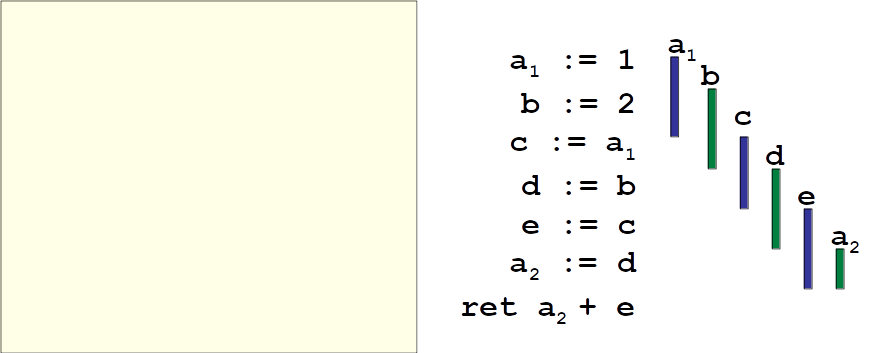
\includegraphics[width=0.9\paperwidth]{figures/quiz2}
%\end{figure}
%\end{frame}

\section{Стандартные алгоритмы (prior work)} 


\begin{frame}{Стандартные алгоритмы (1/2)}
\begin{itemize}
\item Раскраска вершин графа в k цветов (Chaitin et al. 1982)
\begin{itemize}
\item NP-полная задача
\item требудет live range splitting, иначе spillится слишком много
\item переменная, которая не spilled, всегда находится в одном регистре
\item алгоритмы для оптимизации coalescing слишком консервативны (Briggs)
\end{itemize}

\item Linear Scan Rgister Allocation (2я половина 1990х) -- жадный алгоритм\\
  появился из-за критики консервативных подходов к coalescing
\begin{itemize}
\item Изначально работал существенное быстре, но выдавал не такой хороший код
\item Позже это улучшили с помощью binpacking (Traub et al., 1998)
\item Дальнейшее: выбор более оптимальных место для live range splitting
\item \emph{Extended linear scan} -- вставка дополнительных инструкций для уменьшения spilling
\end{itemize}\end{itemize}
\end{frame}

\begin{frame}{Стандартные алгоритмы (2/2)}
\begin{itemize}
\item Linear Programming -- слишком медленный, даже по сравнению с раскраской графа
\item Register allocation via Partitioned Quadratic Programming\\
  дает оптимальное решение (если оно есть) за $O(\mid\!V\!\mid\cdot K^3)$, где $V$~-- переменные, а $K$~-- количество регистров
  % Хз что там с нерегулярными архитектурами
  
\item Register allocation via Multi-Flow of Commodities\\
  Умеет порождать более маленький код, чем раскраска графа
\item Распределение регистров на основе SSA представления (2005)
\item Распределение регистров с помощью решения паззлов (2008)
\end{itemize}
\end{frame}


\begin{frame}{Распределение регистров на основе SSA представления (2005)}
\begin{itemize}
\item Существенный прогресс
\item Из-за SSA представления программ interference graph можно сделать хордовым
\item Тогда алгоритм раскраски графа становится полиномиальным
\end{itemize}

\begin{definition}[Хордальный граф (сhordal graph)]
Граф называется \emph{хордовым (chordal)}, если каждый из его циклов, имеющих четыре ребра и более, имеет хорду (ребро, соединяющее две вершины цикла, но не являющееся его частью)
\end{definition}
\end{frame}


\begin{frame}[fragile]{}
\begin{figure}
\centering
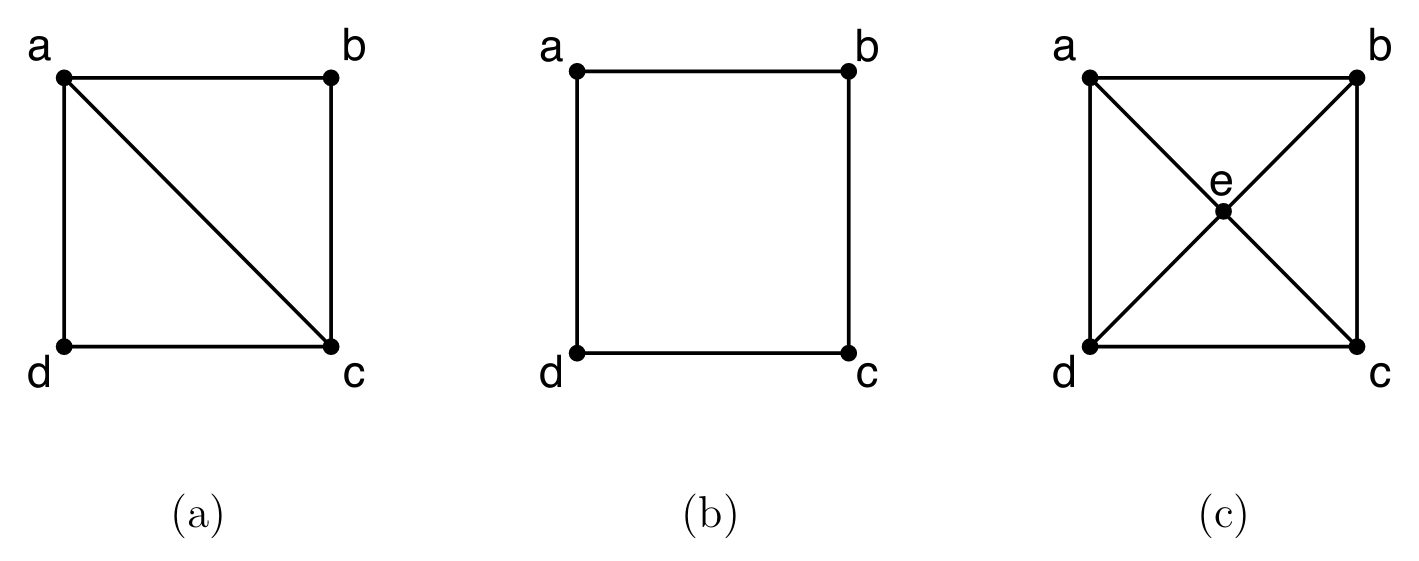
\includegraphics[width=0.9\linewidth]{figures/hordes}
\caption{(a) Хордовый граф. (b-c) Нехордовые графы}
\end{figure}


Ходовые графы имеют хорошие свойства. Задачи \emph{минимальной раскраски},
\emph{поиска максимальной клики} и \emph{минимального покрытия кликами} NP-полны, но решаются за полиномиальное время для хордовых графов. 
%In particular, optimal coloring of a chordal graph G = (V, E)
%can be done in O(|E| + |V |) time.
\end{frame}

\section{Построение элементарных программ}

\begin{frame}[fragile]{Из программ в кусочки паззлов}
\begin{enumerate}
\item[1.] Преобразуем в программу в более простой вид
  \begin{enumerate}
  \item[A.] Преобразуем исходную программу в SSA
  \item[B.] Преобразуем A в SSI форму
  \item[C.] Вставляем в В параллельное копирование между каждой парой инструкций
  \end{enumerate}
\item[2.] Отображаем элементарные программы в кусочки паззлов.
\end{enumerate}
\end{frame}

\subsection{SSA}

\begin{frame}[fragile]{Static Single Assignment (SSA)}

\begin{definition}[SSA форма]
Программа находится в SSA форме, если для всякой переменной только одна инструкция (statement) присваивания в тесте программы присваивает значение этой переменной
\end{definition}

Плюсы:
\begin{itemize}
\item ссылочная прозрачность (referential transparency)
\item значение переменной не зависит от позиции вхождения её идентификатора в программу
\end{itemize}
\end{frame}


\begin{frame}[fragile]{}
\begin{figure}
%\centering
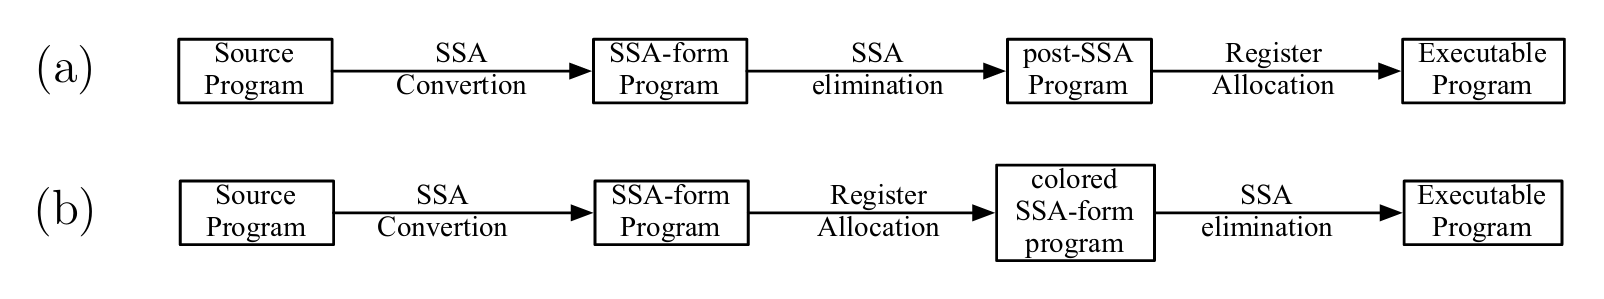
\includegraphics[width=1.0\linewidth]{figures/ssa-compilation-scheme}
\caption{(a) Классическое распределение регистров, (b) Распределение регистров на основе SSA}
\label{fig:ssa-compilation-scheme}
\end{figure}
\end{frame}



\begin{frame}[fragile]{Static Single Assignment (SSA). Пример}
Переменной присваивается значение только один раз
\noindent{
  \begin{minipage}[t]{0.48\linewidth}
  \begin{minted}[]{c}
  /* not a SSA */
  x = 1;
  y = x + 1;
  x = 2;
  z = x + 1;
  \end{minted}
\end{minipage}}
\hfill
\begin{minipage}[t]{0.48\linewidth}
  \begin{minted}[]{c}
  /* SSA */
  x1 = 1;
  y = x1 + 1;
  x2 = 2;
  z = x2 + 1;
  \end{minted}
\end{minipage}\vspace{1em}

В примере выше хочется соптимизировать и написать \mintinline{c}{z = y;} так как правые части синтаксически одинаковые.\\

Но это сделать нельзя так как в \mintinline{c}{x} присваивается новое значение, т.е. содержимое перемернной \mintinline{c}{z} зависит от контекста.\vspace{1em}

\textbf{Мотивация}: хотим \emph{хранить} некоторую информацию \emph{в каждой точке} программы

\end{frame}

\begin{frame}[fragile]{Пример: храним в каждой точке программы информацию о константах}
\begin{center}
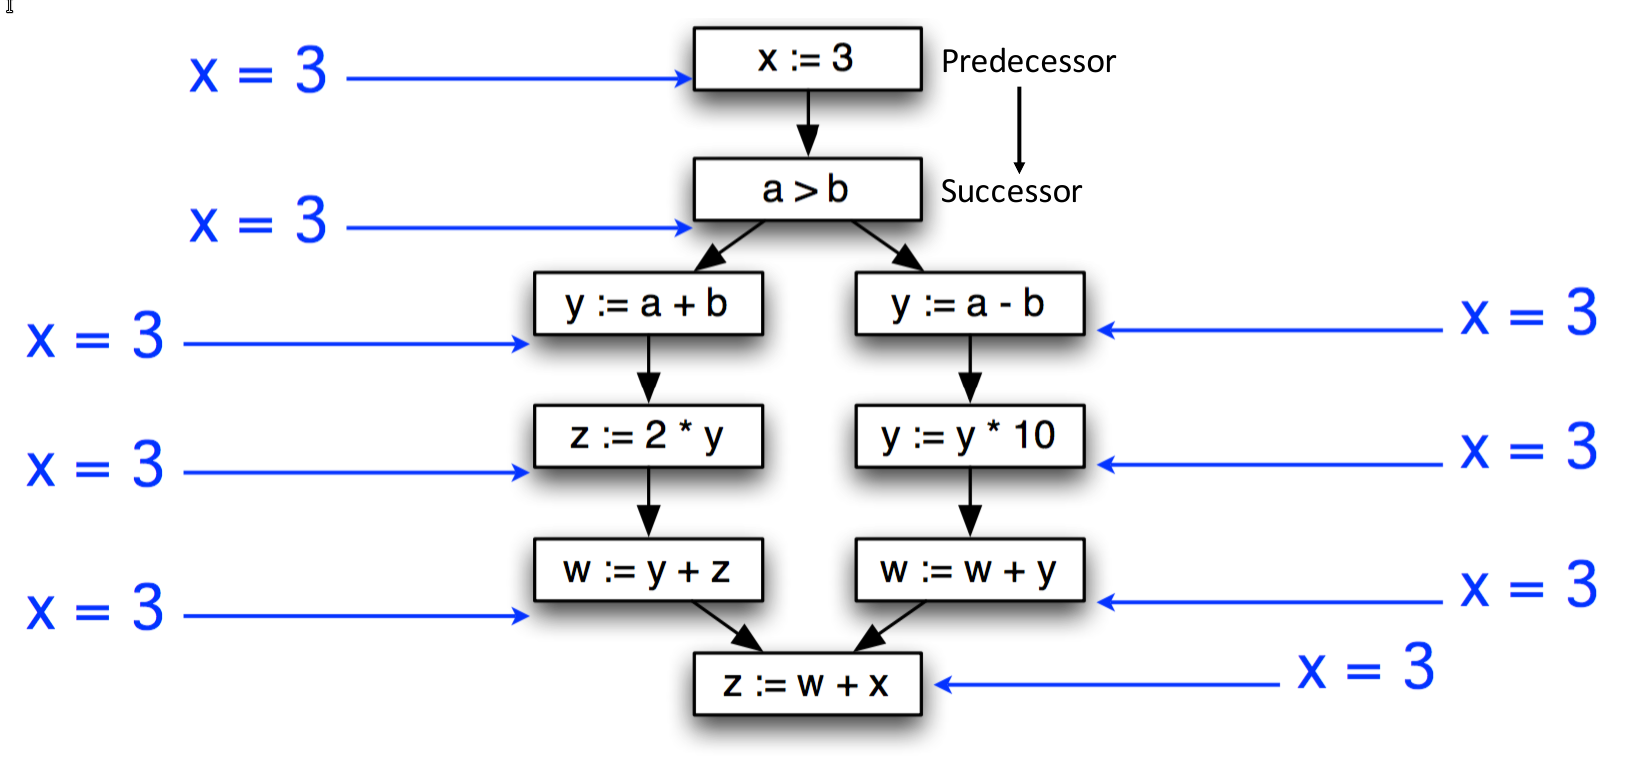
\includegraphics[width=.9\textwidth]{figures/ssa-search-for-constants}
\end{center}
\end{frame}

\tikzstyle{basic block} = [rectangle, rounded corners=3mm, align=left]
\tikzstyle{large bb} = [draw, text width=3cm]
\tikzstyle{very large bb} = [draw, text width=4cm]
\tikzstyle{normal bb} = [draw, text width=2cm]

\begin{frame}[fragile]{Разветвление потока управления (1/2)}
\noindent{
\begin{minipage}[t]{0.48\linewidth}
\begin{minted}[]{c}
  x = input();
  if (x==42)
  then 
    y = 1; /* A */
  else 
    y = x+2; /* B */
  end
  print(y);
\end{minted}
\end{minipage}}
\begin{minipage}[t]{0.48\linewidth}
\begin{figure}
\kern1cm
\begin{tikzpicture}[node distance=1.2cm and -.8cm]
    % Place nodes
    \path (0,0) node  [basic block, large bb] (l1) 
    {$x \leftarrow input()$\\$(x=42)?$ }
    +(-1.8,-2.2) node [basic block, normal bb] (l3) {$y \leftarrow 1$}
    +(+1.8,-2.2) node [basic block, normal bb] (l5) {$y \leftarrow x+2$}
    +(0,-4) node [basic block, large bb] (l7)
        {$print(y)$};

    % Draw edges
    \path [] (l1) edge (l3) edge (l5);
    \path [] (l3) edge (l7);
    \path [] (l5) edge (l7);

%    \increaseshadowboundingbox
\end{tikzpicture}

\end{figure}
\end{minipage}\vspace{1em}

\end{frame}

\begin{frame}[fragile]{Разветвление потока управления (2/2)}
\begin{itemize}
\item Добавляем $\varphi$-функции ($\varphi$-узлы), чтобы смоделировать слияние потоков управления

\item Операционно: выбираем один из аргументов в зависимости откуда пришли
\item Несколько присваиваний $\varphi$-функций должны выполняться \emph{параллельно} (одновременно)
\item При кодогенерации от $\varphi$ надо будет избавляться
\end{itemize}

\noindent{
\begin{minipage}[t]{0.4\linewidth}
\begin{minted}[escapeinside=??]{c}
  x = input();
  if (x==42)
  then 
    ?$y_1$? = 1; /* A */
  else 
    ?$y_2$? = x+2; /* B */
  end
  ?$y_3$? = ?$\varphi(y_1,y_2);$?
  print(?$y_3$?);
\end{minted}
\end{minipage}}
\begin{minipage}[t]{0.52\linewidth}
\begin{figure}
\kern1cm
\begin{tikzpicture}[node distance=1.2cm and -.8cm]
    % Place nodes
    \path (0,0) node  [basic block, large bb] (l1) 
                       {$x \leftarrow input()$\\$(x=42)?$ }
    +(-1.8,-2.2) node [basic block, normal bb] (l3) {$y_1 \leftarrow 1$}
    +(+1.8,-2.2) node [basic block, normal bb] (l5) {$y_2 \leftarrow x+2$}
    +(0,-4) node [basic block, very large bb] (l7)
        {$y3\leftarrow \varphi(A:y_1, B:y_2)$\\$print(y_3)$};

    % Draw edges
    \path [] (l1) edge (l3) edge (l5);
    \path [] (l3) edge (l7);
    \path [] (l5) edge (l7);

%    \increaseshadowboundingbox
\end{tikzpicture}

\end{figure}
\end{minipage}

\end{frame}


\begin{frame}[fragile]
\begin{figure}
\centering
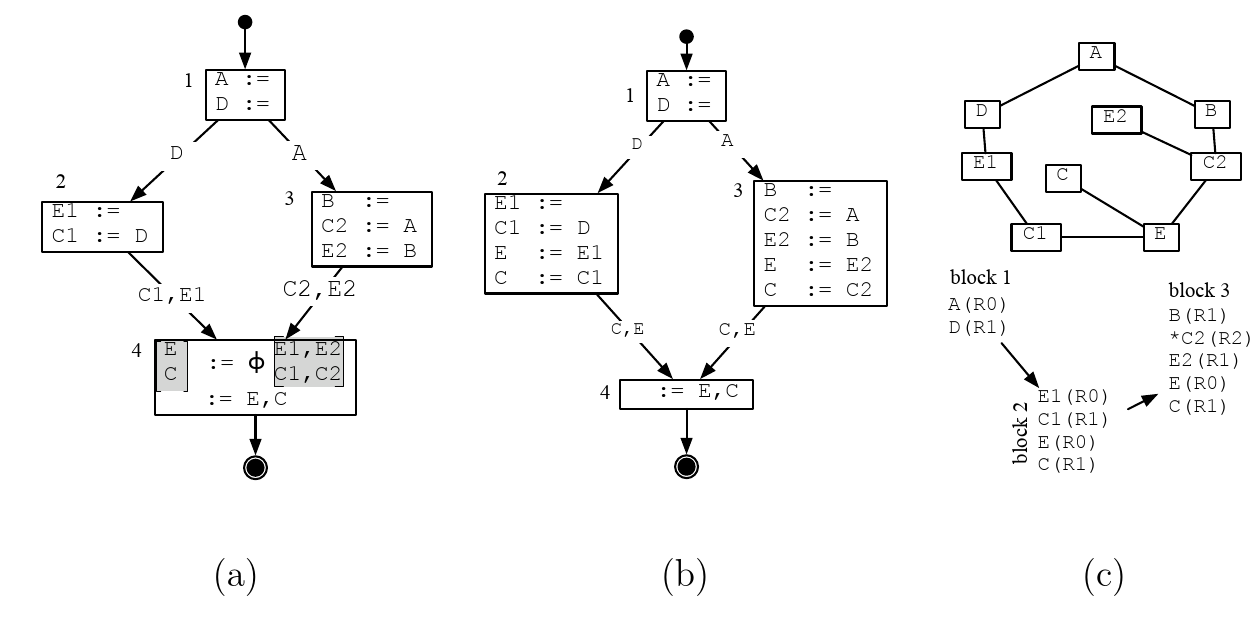
\includegraphics[width=.9\textwidth]{figures/regalloc-ssa}
\caption{ (a) SSA-форма программы . 
(b) Программа после избавления от SSA. 
(c) Граф несовместимости и последовательность присвоений в регистры }
\end{figure}
\end{frame}

\begin{frame}[fragile]{Избавляемся от  $\varphi$-функций}
Основная идея: $\varphi$ обозначает тот факт, что значение при слиянии потоков управления может прийти по различным путям управления
\begin{itemize}
\item Сделаем присваивание на каждом пути управления
\item Несколько присваиваний $\varphi$-функций выполняется одновременно
\end{itemize}
\begin{figure}
\centering


\tikzset{every picture/.style={line width=0.75pt}} %set default line width to 0.75pt        

\begin{tikzpicture}[x=0.75pt,y=0.75pt,yscale=-1,xscale=1]
%uncomment if require: \path (0,139.6999969482422); %set diagram left start at 0, and has height of 139.6999969482422

%Rounded Rect [id:dp262243382651531] 
\draw   (10,20.6) .. controls (10,16.4) and (13.4,13) .. (17.6,13) -- (75.9,13) .. controls (80.1,13) and (83.5,16.4) .. (83.5,20.6) -- (83.5,43.4) .. controls (83.5,47.6) and (80.1,51) .. (75.9,51) -- (17.6,51) .. controls (13.4,51) and (10,47.6) .. (10,43.4) -- cycle ;
%Rounded Rect [id:dp4192314773958711] 
\draw   (96.5,19.6) .. controls (96.5,15.4) and (99.9,12) .. (104.1,12) -- (162.4,12) .. controls (166.6,12) and (170,15.4) .. (170,19.6) -- (170,42.4) .. controls (170,46.6) and (166.6,50) .. (162.4,50) -- (104.1,50) .. controls (99.9,50) and (96.5,46.6) .. (96.5,42.4) -- cycle ;
%Rounded Rect [id:dp14874696406611254] 
\draw   (40,89.6) .. controls (40,85.4) and (43.4,82) .. (47.6,82) -- (141.15,82) .. controls (145.35,82) and (148.75,85.4) .. (148.75,89.6) -- (148.75,112.4) .. controls (148.75,116.6) and (145.35,120) .. (141.15,120) -- (47.6,120) .. controls (43.4,120) and (40,116.6) .. (40,112.4) -- cycle ;
%Straight Lines [id:da8036054523449865] 
\draw    (50,50) -- (98.29,78.97) ;
\draw [shift={(100,80)}, rotate = 210.96] [color={rgb, 255:red, 0; green, 0; blue, 0 }  ][line width=0.75]    (10.93,-3.29) .. controls (6.95,-1.4) and (3.31,-0.3) .. (0,0) .. controls (3.31,0.3) and (6.95,1.4) .. (10.93,3.29)   ;

%Straight Lines [id:da9462543361304327] 
\draw    (130,50) -- (101.41,78.59) ;
\draw [shift={(100,80)}, rotate = 315] [color={rgb, 255:red, 0; green, 0; blue, 0 }  ][line width=0.75]    (10.93,-3.29) .. controls (6.95,-1.4) and (3.31,-0.3) .. (0,0) .. controls (3.31,0.3) and (6.95,1.4) .. (10.93,3.29)   ;

%Right Arrow [id:dp5454010361665674] 
\draw   (200,50) -- (242,50) -- (242,40) -- (270,60) -- (242,80) -- (242,70) -- (200,70) -- cycle ;
%Rounded Rect [id:dp804370127764321] 
\draw   (280,18.6) .. controls (280,14.4) and (283.4,11) .. (287.6,11) -- (345.9,11) .. controls (350.1,11) and (353.5,14.4) .. (353.5,18.6) -- (353.5,41.4) .. controls (353.5,45.6) and (350.1,49) .. (345.9,49) -- (287.6,49) .. controls (283.4,49) and (280,45.6) .. (280,41.4) -- cycle ;
%Rounded Rect [id:dp054537017000311994] 
\draw   (366.5,17.6) .. controls (366.5,13.4) and (369.9,10) .. (374.1,10) -- (432.4,10) .. controls (436.6,10) and (440,13.4) .. (440,17.6) -- (440,40.4) .. controls (440,44.6) and (436.6,48) .. (432.4,48) -- (374.1,48) .. controls (369.9,48) and (366.5,44.6) .. (366.5,40.4) -- cycle ;
%Rounded Rect [id:dp9347541053691467] 
\draw   (310,87.6) .. controls (310,83.4) and (313.4,80) .. (317.6,80) -- (411.15,80) .. controls (415.35,80) and (418.75,83.4) .. (418.75,87.6) -- (418.75,110.4) .. controls (418.75,114.6) and (415.35,118) .. (411.15,118) -- (317.6,118) .. controls (313.4,118) and (310,114.6) .. (310,110.4) -- cycle ;
%Straight Lines [id:da09161146890023963] 
\draw    (320,48) -- (368.29,76.97) ;
\draw [shift={(370,78)}, rotate = 210.96] [color={rgb, 255:red, 0; green, 0; blue, 0 }  ][line width=0.75]    (10.93,-3.29) .. controls (6.95,-1.4) and (3.31,-0.3) .. (0,0) .. controls (3.31,0.3) and (6.95,1.4) .. (10.93,3.29)   ;

%Straight Lines [id:da9445970974561072] 
\draw    (400,48) -- (371.41,76.59) ;
\draw [shift={(370,78)}, rotate = 315] [color={rgb, 255:red, 0; green, 0; blue, 0 }  ][line width=0.75]    (10.93,-3.29) .. controls (6.95,-1.4) and (3.31,-0.3) .. (0,0) .. controls (3.31,0.3) and (6.95,1.4) .. (10.93,3.29)   ;


% Text Node
\draw (46.75,32) node  [align=left] {{\fontfamily{pcr}\selectfont b1=c+1}};
% Text Node
\draw (133.25,31) node  [align=left] {{\fontfamily{pcr}\selectfont b2=d+1}};
% Text Node
\draw (94.38,101) node  [align=left] {{\fontfamily{pcr}\selectfont b3=$\varphi$(b1,b2)}\\{\fontfamily{pcr}\selectfont if (b3>N)}};
% Text Node
\draw (316.75,30) node  [align=left] {{\fontfamily{pcr}\selectfont b1=c+1}\\{\fontfamily{pcr}\selectfont b3=b1}};
% Text Node
\draw (403.25,29) node  [align=left] {{\fontfamily{pcr}\selectfont b2=d+1}\\{\fontfamily{pcr}\selectfont b3=b2}};
% Text Node
\draw (364.38,99) node  [align=left] {{\fontfamily{pcr}\selectfont if (b3>N)}};

\draw (100,140) node  [align=left] {\textcolor{teal}{SSA}};
\draw (364,140) node  [align=left] {\textcolor{red}{Не SSA}};


\end{tikzpicture}

\end{figure}
\end{frame}

\begin{frame}[fragile]{Избавляемся от $\varphi$ на практике}
\begin{itemize}
\item Копирования из-за $\varphi$ могут быть бесполезны
\item Объединенное (joined) значение может быть не нужно далее в программе (зачем его оставлять?)
\item Воспользуемся dead code elimination, чтобы убрать бесполезные $\varphi$
\item Затем будет заниматься распределением регистров
\end{itemize}
\end{frame}


\begin{frame}[fragile]{Про NP-полноту}
Задача Spill Free Register Allocation (SFRA) для SSA формы имеет полиномиальное решение, но NP-полно в общем случае.\\

% Any program can be converted into SSA-form via a polynomial time
%transformation [27]. However, a register assignment for a SSA-form program can-
%not be converted back to an optimal register assignment of the original program
%in polynomial time unless P=NP.

Большое количество полезных задач NP-полно для SSA формы, а следовательно NP-полно для всех программ
\begin{itemize}
\item Spill minimization
\item (Optimal) Coalescing
\item (Optimal) Live range splitting 
\item (Optimal) aliasing
\item Pre-coloring
\end{itemize}
Можно попробовать использовать более простое представление программ, чтобы получались полиномиальные алгоритмы
\end{frame}

\subsection{SSI}

\begin{frame}[fragile]{Static Single Information (SSI)}
По умолчанию SSA связывает некоторую информацию с парой переменная $\times$ позиция в программе -- это \emph{плотный (dense) анализ}.\\

Для некоторых видов анализа будет удобнее связывать иметь общую информацию по всей программе с конкретной переменной, а не каждым её вхождением (\emph{sparse анализ}). \\

Это удобно для таких анализов:
\begin{itemize}
\item вывод классов с виртуальными методами по классам-таблицам (Python, Javascript, Ruby) % \& Lua)
\item Null pointer анализ
\item интервалы значений (далее будет пример)
\item live range splitting (важно в контексте выделения регистров)
\end{itemize}
\end{frame}

\begin{frame}[fragile]{Пример плотного data-flow анализа: интервальный анализ}
\begin{figure}
\centering
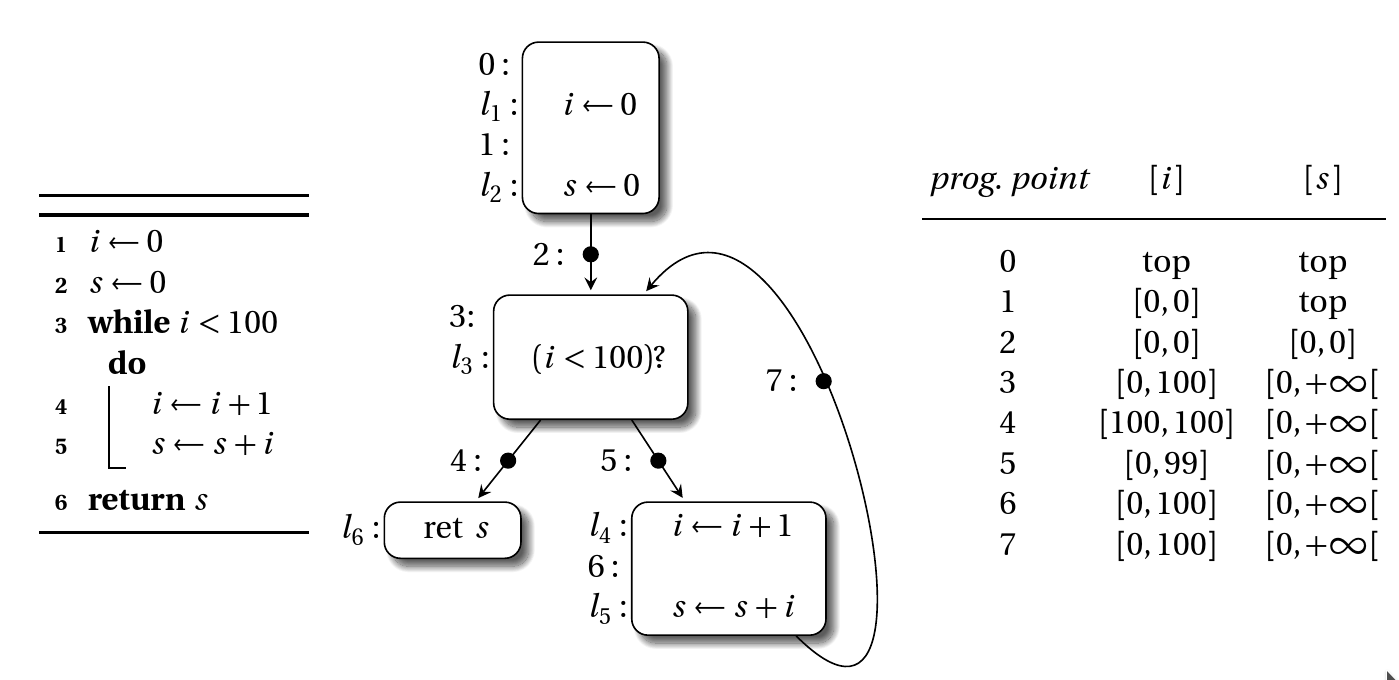
\includegraphics[height=.85\textheight]{figures/dense-range-analysis}
\end{figure}
%An example of a dense data-flow analysis that finds the range of possible values associated
%with each variable at each program point.
\end{frame}

\begin{frame}[fragile]{Static Single Information (SSI) форма}
Программа в SSI форме:
\begin{itemize}
\item Каждый базовый блок заканчивается π-функцией, которая переименовывает переменные, которые ``живы`` на выходе из базового блока
\end{itemize}

\begin{figure}
\centering


\tikzset{every picture/.style={line width=0.75pt}} %set default line width to 0.75pt        

\begin{tikzpicture}[x=0.75pt,y=0.75pt,yscale=-1,xscale=1]
%uncomment if require: \path (0,139.6999969482422); %set diagram left start at 0, and has height of 139.6999969482422

%Rounded Rect [id:dp262243382651531] 
\draw   (10,99.6) .. controls (10,95.4) and (13.4,92) .. (17.6,92) -- (75.9,92) .. controls (80.1,92) and (83.5,95.4) .. (83.5,99.6) -- (83.5,122.4) .. controls (83.5,126.6) and (80.1,130) .. (75.9,130) -- (17.6,130) .. controls (13.4,130) and (10,126.6) .. (10,122.4) -- cycle ;
%Rounded Rect [id:dp4192314773958711] 
\draw   (96.5,98.6) .. controls (96.5,94.4) and (99.9,91) .. (104.1,91) -- (162.4,91) .. controls (166.6,91) and (170,94.4) .. (170,98.6) -- (170,121.4) .. controls (170,125.6) and (166.6,129) .. (162.4,129) -- (104.1,129) .. controls (99.9,129) and (96.5,125.6) .. (96.5,121.4) -- cycle ;
%Rounded Rect [id:dp14874696406611254] 
\draw   (20,20.6) .. controls (20,16.4) and (23.4,13) .. (27.6,13) -- (121.15,13) .. controls (125.35,13) and (128.75,16.4) .. (128.75,20.6) -- (128.75,43.4) .. controls (128.75,47.6) and (125.35,51) .. (121.15,51) -- (27.6,51) .. controls (23.4,51) and (20,47.6) .. (20,43.4) -- cycle ;
%Straight Lines [id:da8036054523449865] 
\draw    (80,51) -- (51.2,89.4) ;
\draw [shift={(50,91)}, rotate = 306.87] [color={rgb, 255:red, 0; green, 0; blue, 0 }  ][line width=0.75]    (10.93,-3.29) .. controls (6.95,-1.4) and (3.31,-0.3) .. (0,0) .. controls (3.31,0.3) and (6.95,1.4) .. (10.93,3.29)   ;

%Straight Lines [id:da9462543361304327] 
\draw    (80,51) -- (118.59,89.59) ;
\draw [shift={(120,91)}, rotate = 225] [color={rgb, 255:red, 0; green, 0; blue, 0 }  ][line width=0.75]    (10.93,-3.29) .. controls (6.95,-1.4) and (3.31,-0.3) .. (0,0) .. controls (3.31,0.3) and (6.95,1.4) .. (10.93,3.29)   ;

%Right Arrow [id:dp5454010361665674] 
\draw   (180,51) -- (222,51) -- (222,41) -- (250,61) -- (222,81) -- (222,71) -- (180,71) -- cycle ;
%Rounded Rect [id:dp804370127764321] 
\draw   (270,99.6) .. controls (270,95.4) and (273.4,92) .. (277.6,92) -- (335.9,92) .. controls (340.1,92) and (343.5,95.4) .. (343.5,99.6) -- (343.5,122.4) .. controls (343.5,126.6) and (340.1,130) .. (335.9,130) -- (277.6,130) .. controls (273.4,130) and (270,126.6) .. (270,122.4) -- cycle ;
%Rounded Rect [id:dp054537017000311994] 
\draw   (356.5,98.6) .. controls (356.5,94.4) and (359.9,91) .. (364.1,91) -- (422.4,91) .. controls (426.6,91) and (430,94.4) .. (430,98.6) -- (430,121.4) .. controls (430,125.6) and (426.6,129) .. (422.4,129) -- (364.1,129) .. controls (359.9,129) and (356.5,125.6) .. (356.5,121.4) -- cycle ;
%Rounded Rect [id:dp9347541053691467] 
\draw   (290,18.6) .. controls (290,14.4) and (293.4,11) .. (297.6,11) -- (391.15,11) .. controls (395.35,11) and (398.75,14.4) .. (398.75,18.6) -- (398.75,41.4) .. controls (398.75,45.6) and (395.35,49) .. (391.15,49) -- (297.6,49) .. controls (293.4,49) and (290,45.6) .. (290,41.4) -- cycle ;
%Straight Lines [id:da09161146890023963] 
\draw    (340,51) -- (311.2,89.4) ;
\draw [shift={(310,91)}, rotate = 306.87] [color={rgb, 255:red, 0; green, 0; blue, 0 }  ][line width=0.75]    (10.93,-3.29) .. controls (6.95,-1.4) and (3.31,-0.3) .. (0,0) .. controls (3.31,0.3) and (6.95,1.4) .. (10.93,3.29)   ;

%Straight Lines [id:da9445970974561072] 
\draw    (340,51) -- (388.44,89.75) ;
\draw [shift={(390,91)}, rotate = 218.66] [color={rgb, 255:red, 0; green, 0; blue, 0 }  ][line width=0.75]    (10.93,-3.29) .. controls (6.95,-1.4) and (3.31,-0.3) .. (0,0) .. controls (3.31,0.3) and (6.95,1.4) .. (10.93,3.29)   ;


% Text Node
\draw (46.75,111) node  [align=left] {{\tt ...=c+1}};
% Text Node
\draw (133.25,110) node  [align=left] {{\tt ...=c*2}};
% Text Node
\draw (74.38,32) node  [align=left] {{\tt if (b>1)}};
% Text Node
\draw (344.38,30) node  [align=left] {{\tt if (b>1)}\\{\tt (c1,c2)=$\pi$(c)}};
% Text Node
\draw (309,111.5) node  [align=left] {{\tt ...=c1+1}};
% Text Node
\draw (393.25,110) node  [align=left] {{\tt ...=c2*2}};

\draw (90,160) node  [align=left] {\textcolor{red}{не SSI}};
\draw (350,160) node  [align=left] {\textcolor{teal}{SSI}};
\end{tikzpicture}

\end{figure}
\emph{Базовый блок} -- это последовательность инструкций с только одной точкой входа и только одной точкой выхода.
\end{frame}

\begin{frame}[fragile]{Примеры SSA и SSI}
\begin{figure}
\centering


\tikzset{every picture/.style={line width=0.75pt}} %set default line width to 0.75pt        

\begin{tikzpicture}[x=0.75pt,y=0.75pt,yscale=-1,xscale=1]
%uncomment if require: \path (0,314.6999969482422); %set diagram left start at 0, and has height of 314.6999969482422

%Rounded Rect [id:dp262243382651531] 
\draw   (10,188.6) .. controls (10,184.4) and (13.4,181) .. (17.6,181) -- (75.9,181) .. controls (80.1,181) and (83.5,184.4) .. (83.5,188.6) -- (83.5,211.4) .. controls (83.5,215.6) and (80.1,219) .. (75.9,219) -- (17.6,219) .. controls (13.4,219) and (10,215.6) .. (10,211.4) -- cycle ;
%Rounded Rect [id:dp4192314773958711] 
\draw   (96.5,187.6) .. controls (96.5,183.4) and (99.9,180) .. (104.1,180) -- (162.4,180) .. controls (166.6,180) and (170,183.4) .. (170,187.6) -- (170,210.4) .. controls (170,214.6) and (166.6,218) .. (162.4,218) -- (104.1,218) .. controls (99.9,218) and (96.5,214.6) .. (96.5,210.4) -- cycle ;
%Rounded Rect [id:dp14874696406611254] 
\draw   (30,93.6) .. controls (30,87.19) and (35.19,82) .. (41.6,82) -- (127.15,82) .. controls (133.56,82) and (138.75,87.19) .. (138.75,93.6) -- (138.75,128.4) .. controls (138.75,134.81) and (133.56,140) .. (127.15,140) -- (41.6,140) .. controls (35.19,140) and (30,134.81) .. (30,128.4) -- cycle ;
%Straight Lines [id:da8036054523449865] 
\draw    (80,140) -- (51.2,178.4) ;
\draw [shift={(50,180)}, rotate = 306.87] [color={rgb, 255:red, 0; green, 0; blue, 0 }  ][line width=0.75]    (10.93,-3.29) .. controls (6.95,-1.4) and (3.31,-0.3) .. (0,0) .. controls (3.31,0.3) and (6.95,1.4) .. (10.93,3.29)   ;

%Straight Lines [id:da9462543361304327] 
\draw    (80,140) -- (118.59,178.59) ;
\draw [shift={(120,180)}, rotate = 225] [color={rgb, 255:red, 0; green, 0; blue, 0 }  ][line width=0.75]    (10.93,-3.29) .. controls (6.95,-1.4) and (3.31,-0.3) .. (0,0) .. controls (3.31,0.3) and (6.95,1.4) .. (10.93,3.29)   ;

%Rounded Rect [id:dp804370127764321] 
\draw   (190,187.6) .. controls (190,183.4) and (193.4,180) .. (197.6,180) -- (255.9,180) .. controls (260.1,180) and (263.5,183.4) .. (263.5,187.6) -- (263.5,210.4) .. controls (263.5,214.6) and (260.1,218) .. (255.9,218) -- (197.6,218) .. controls (193.4,218) and (190,214.6) .. (190,210.4) -- cycle ;
%Rounded Rect [id:dp054537017000311994] 
\draw   (276.5,186.6) .. controls (276.5,182.4) and (279.9,179) .. (284.1,179) -- (342.4,179) .. controls (346.6,179) and (350,182.4) .. (350,186.6) -- (350,209.4) .. controls (350,213.6) and (346.6,217) .. (342.4,217) -- (284.1,217) .. controls (279.9,217) and (276.5,213.6) .. (276.5,209.4) -- cycle ;
%Rounded Rect [id:dp9347541053691467] 
\draw   (210,91) .. controls (210,84.37) and (215.37,79) .. (222,79) -- (306.75,79) .. controls (313.38,79) and (318.75,84.37) .. (318.75,91) -- (318.75,127) .. controls (318.75,133.63) and (313.38,139) .. (306.75,139) -- (222,139) .. controls (215.37,139) and (210,133.63) .. (210,127) -- cycle ;
%Straight Lines [id:da09161146890023963] 
\draw    (260,139) -- (231.2,177.4) ;
\draw [shift={(230,179)}, rotate = 306.87] [color={rgb, 255:red, 0; green, 0; blue, 0 }  ][line width=0.75]    (10.93,-3.29) .. controls (6.95,-1.4) and (3.31,-0.3) .. (0,0) .. controls (3.31,0.3) and (6.95,1.4) .. (10.93,3.29)   ;

%Straight Lines [id:da9445970974561072] 
\draw    (260,139) -- (308.44,177.75) ;
\draw [shift={(310,179)}, rotate = 218.66] [color={rgb, 255:red, 0; green, 0; blue, 0 }  ][line width=0.75]    (10.93,-3.29) .. controls (6.95,-1.4) and (3.31,-0.3) .. (0,0) .. controls (3.31,0.3) and (6.95,1.4) .. (10.93,3.29)   ;

%Rounded Rect [id:dp4977532430387589] 
\draw   (10,19.6) .. controls (10,15.4) and (13.4,12) .. (17.6,12) -- (75.9,12) .. controls (80.1,12) and (83.5,15.4) .. (83.5,19.6) -- (83.5,42.4) .. controls (83.5,46.6) and (80.1,50) .. (75.9,50) -- (17.6,50) .. controls (13.4,50) and (10,46.6) .. (10,42.4) -- cycle ;
%Rounded Rect [id:dp5889626886983321] 
\draw   (96.5,18.6) .. controls (96.5,14.4) and (99.9,11) .. (104.1,11) -- (162.4,11) .. controls (166.6,11) and (170,14.4) .. (170,18.6) -- (170,41.4) .. controls (170,45.6) and (166.6,49) .. (162.4,49) -- (104.1,49) .. controls (99.9,49) and (96.5,45.6) .. (96.5,41.4) -- cycle ;
%Straight Lines [id:da038881567998766964] 
\draw    (50,50) -- (88.4,78.8) ;
\draw [shift={(90,80)}, rotate = 216.87] [color={rgb, 255:red, 0; green, 0; blue, 0 }  ][line width=0.75]    (10.93,-3.29) .. controls (6.95,-1.4) and (3.31,-0.3) .. (0,0) .. controls (3.31,0.3) and (6.95,1.4) .. (10.93,3.29)   ;

%Straight Lines [id:da9119956977469609] 
\draw    (130,50) -- (91.6,78.8) ;
\draw [shift={(90,80)}, rotate = 323.13] [color={rgb, 255:red, 0; green, 0; blue, 0 }  ][line width=0.75]    (10.93,-3.29) .. controls (6.95,-1.4) and (3.31,-0.3) .. (0,0) .. controls (3.31,0.3) and (6.95,1.4) .. (10.93,3.29)   ;

%Rounded Rect [id:dp450867564409416] 
\draw   (190,18.6) .. controls (190,14.4) and (193.4,11) .. (197.6,11) -- (255.9,11) .. controls (260.1,11) and (263.5,14.4) .. (263.5,18.6) -- (263.5,41.4) .. controls (263.5,45.6) and (260.1,49) .. (255.9,49) -- (197.6,49) .. controls (193.4,49) and (190,45.6) .. (190,41.4) -- cycle ;
%Rounded Rect [id:dp06195868427554574] 
\draw   (276.5,17.6) .. controls (276.5,13.4) and (279.9,10) .. (284.1,10) -- (342.4,10) .. controls (346.6,10) and (350,13.4) .. (350,17.6) -- (350,40.4) .. controls (350,44.6) and (346.6,48) .. (342.4,48) -- (284.1,48) .. controls (279.9,48) and (276.5,44.6) .. (276.5,40.4) -- cycle ;
%Straight Lines [id:da334726632196392] 
\draw    (230,49) -- (268.4,77.8) ;
\draw [shift={(270,79)}, rotate = 216.87] [color={rgb, 255:red, 0; green, 0; blue, 0 }  ][line width=0.75]    (10.93,-3.29) .. controls (6.95,-1.4) and (3.31,-0.3) .. (0,0) .. controls (3.31,0.3) and (6.95,1.4) .. (10.93,3.29)   ;

%Straight Lines [id:da41014358467548495] 
\draw    (310,49) -- (271.6,77.8) ;
\draw [shift={(270,79)}, rotate = 323.13] [color={rgb, 255:red, 0; green, 0; blue, 0 }  ][line width=0.75]    (10.93,-3.29) .. controls (6.95,-1.4) and (3.31,-0.3) .. (0,0) .. controls (3.31,0.3) and (6.95,1.4) .. (10.93,3.29)   ;

%Rounded Rect [id:dp3691248800233007] 
\draw   (360,187.6) .. controls (360,183.4) and (363.4,180) .. (367.6,180) -- (425.9,180) .. controls (430.1,180) and (433.5,183.4) .. (433.5,187.6) -- (433.5,210.4) .. controls (433.5,214.6) and (430.1,218) .. (425.9,218) -- (367.6,218) .. controls (363.4,218) and (360,214.6) .. (360,210.4) -- cycle ;
%Rounded Rect [id:dp19131836124451396] 
\draw   (446.5,186.6) .. controls (446.5,182.4) and (449.9,179) .. (454.1,179) -- (512.4,179) .. controls (516.6,179) and (520,182.4) .. (520,186.6) -- (520,209.4) .. controls (520,213.6) and (516.6,217) .. (512.4,217) -- (454.1,217) .. controls (449.9,217) and (446.5,213.6) .. (446.5,209.4) -- cycle ;
%Rounded Rect [id:dp14926613816841217] 
\draw   (380,93.2) .. controls (380,85.36) and (386.36,79) .. (394.2,79) -- (474.55,79) .. controls (482.39,79) and (488.75,85.36) .. (488.75,93.2) -- (488.75,135.8) .. controls (488.75,143.64) and (482.39,150) .. (474.55,150) -- (394.2,150) .. controls (386.36,150) and (380,143.64) .. (380,135.8) -- cycle ;
%Straight Lines [id:da6856746540157947] 
\draw    (440,150) -- (401.6,178.8) ;
\draw [shift={(400,180)}, rotate = 323.13] [color={rgb, 255:red, 0; green, 0; blue, 0 }  ][line width=0.75]    (10.93,-3.29) .. controls (6.95,-1.4) and (3.31,-0.3) .. (0,0) .. controls (3.31,0.3) and (6.95,1.4) .. (10.93,3.29)   ;

%Straight Lines [id:da6670526861113566] 
\draw    (440,150) -- (478.4,178.8) ;
\draw [shift={(480,180)}, rotate = 216.87] [color={rgb, 255:red, 0; green, 0; blue, 0 }  ][line width=0.75]    (10.93,-3.29) .. controls (6.95,-1.4) and (3.31,-0.3) .. (0,0) .. controls (3.31,0.3) and (6.95,1.4) .. (10.93,3.29)   ;

%Rounded Rect [id:dp00671566926016387] 
\draw   (360,18.6) .. controls (360,14.4) and (363.4,11) .. (367.6,11) -- (425.9,11) .. controls (430.1,11) and (433.5,14.4) .. (433.5,18.6) -- (433.5,41.4) .. controls (433.5,45.6) and (430.1,49) .. (425.9,49) -- (367.6,49) .. controls (363.4,49) and (360,45.6) .. (360,41.4) -- cycle ;
%Rounded Rect [id:dp8281541882214426] 
\draw   (446.5,17.6) .. controls (446.5,13.4) and (449.9,10) .. (454.1,10) -- (512.4,10) .. controls (516.6,10) and (520,13.4) .. (520,17.6) -- (520,40.4) .. controls (520,44.6) and (516.6,48) .. (512.4,48) -- (454.1,48) .. controls (449.9,48) and (446.5,44.6) .. (446.5,40.4) -- cycle ;
%Straight Lines [id:da8015873618397712] 
\draw    (400,49) -- (438.4,77.8) ;
\draw [shift={(440,79)}, rotate = 216.87] [color={rgb, 255:red, 0; green, 0; blue, 0 }  ][line width=0.75]    (10.93,-3.29) .. controls (6.95,-1.4) and (3.31,-0.3) .. (0,0) .. controls (3.31,0.3) and (6.95,1.4) .. (10.93,3.29)   ;

%Straight Lines [id:da2656759697778148] 
\draw    (480,49) -- (441.6,77.8) ;
\draw [shift={(440,79)}, rotate = 323.13] [color={rgb, 255:red, 0; green, 0; blue, 0 }  ][line width=0.75]    (10.93,-3.29) .. controls (6.95,-1.4) and (3.31,-0.3) .. (0,0) .. controls (3.31,0.3) and (6.95,1.4) .. (10.93,3.29)   ;


% Text Node
\draw (46.75,200) node  [align=left] {{\tt ...=c+1}};
% Text Node
\draw (133.25,199) node  [align=left] {{\tt ...=c*2}};
% Text Node
\draw (84.38,111) node  [align=left] {{\tt if (b>1)}};
% Text Node
\draw (264.38,109) node  [align=left] {{\tt b3 = }$\displaystyle \varphi ${\tt (b1,b2)}\\{\tt if (b3 > 1)}};
% Text Node
\draw (229,199.5) node  [align=left] {{\tt ...=c1+1}};
% Text Node
\draw (313.25,198) node  [align=left] {{\tt ...=c2*2}};
% Text Node
\draw (46.75,31) node  [align=left] {{\tt b=d+1}};
% Text Node
\draw (133.25,30) node  [align=left] {{\tt b=d+4}};
% Text Node
\draw (226.75,30) node  [align=left] {{\tt b1=d+1}};
% Text Node
\draw (313.25,29) node  [align=left] {{\tt b1=d+4}};
% Text Node
\draw (81,241) node  [align=left] {\textcolor{red}{Не SSA и не SSI}};
% Text Node
\draw (269,241) node  [align=left] {\textcolor{teal}{SSA,} \textcolor{red}{но не SSI}};
% Text Node
\draw (436,109.5) node  [align=left] {{\tt b3 = }$\displaystyle \varphi ${\tt (b1,b2)}\\{\tt if (b3 > 1)}\\{\tt (c1,c2)=}$\displaystyle \pi ${\tt (c)}};
% Text Node
\draw (399,199.5) node  [align=left] {{\tt ...=c1+1}};
% Text Node
\draw (483.25,198) node  [align=left] {{\tt ...=c2*2}};
% Text Node
\draw (396.75,30) node  [align=left] {{\tt b1=d+1}};
% Text Node
\draw (483.25,29) node  [align=left] {{\tt b1=d+4}};
% Text Node
\draw (439,241) node  [align=left] {\textcolor{teal}{SSA и SSI}};


\end{tikzpicture}

\end{figure}
\end{frame}


\begin{frame}[fragile]{Параллельное копирование}
По тем же причинам, по которым несколько $\varphi$-функций должны исполняться параллельно, копирование тоже должно происходить параллельно
\begin{figure}
\centering
  
  
  \tikzset{every picture/.style={line width=0.75pt}} %set default line width to 0.75pt        
  
  \begin{tikzpicture}[x=0.75pt,y=0.75pt,yscale=-1,xscale=1]
  %uncomment if require: \path (0,300); %set diagram left start at 0, and has height of 300
  
  %Rounded Rect [id:dp257541138848127] 
  \draw   (7,42.75) .. controls (7,37.33) and (11.39,32.93) .. (16.81,32.93) -- (86.94,32.93) .. controls (92.36,32.93) and (96.75,37.33) .. (96.75,42.75) -- (96.75,72.19) .. controls (96.75,77.61) and (92.36,82) .. (86.94,82) -- (16.81,82) .. controls (11.39,82) and (7,77.61) .. (7,72.19) -- cycle ;
  %Right Arrow [id:dp5774776776599181] 
  \draw   (106,46) -- (148,46) -- (148,36) -- (176,56) -- (148,76) -- (148,66) -- (106,66) -- cycle ;
  %Rounded Rect [id:dp9338900489566466] 
  \draw   (181,26.55) .. controls (181,16.27) and (189.33,7.93) .. (199.61,7.93) -- (578.14,7.93) .. controls (588.42,7.93) and (596.75,16.27) .. (596.75,26.55) -- (596.75,82.39) .. controls (596.75,92.67) and (588.42,101) .. (578.14,101) -- (199.61,101) .. controls (189.33,101) and (181,92.67) .. (181,82.39) -- cycle ;
  
  % Text Node
  \draw (51.88,57.47) node  [align=left] {{\tt V = X + Y}\\{\tt Z = A + B}};
  % Text Node
  \draw (388.38,54.47) node  [align=left] {
    {\tt (V1, X1, Y1, Z1, A1, B1) = (V, X, Y, Z, A, B)}\\
    {\tt V1 = X1 + Y1}\\
    {\tt (V2, X2, Y2, Z2, A2, B2) = (V1, X1, Y1, Z1, A1, B1)}\\
    {\tt Z2 \ = A2 + \ B2}
  };
  
  
  \end{tikzpicture}
  
\end{figure}
\end{frame}


\begin{frame}[fragile]{}
\begin{center}
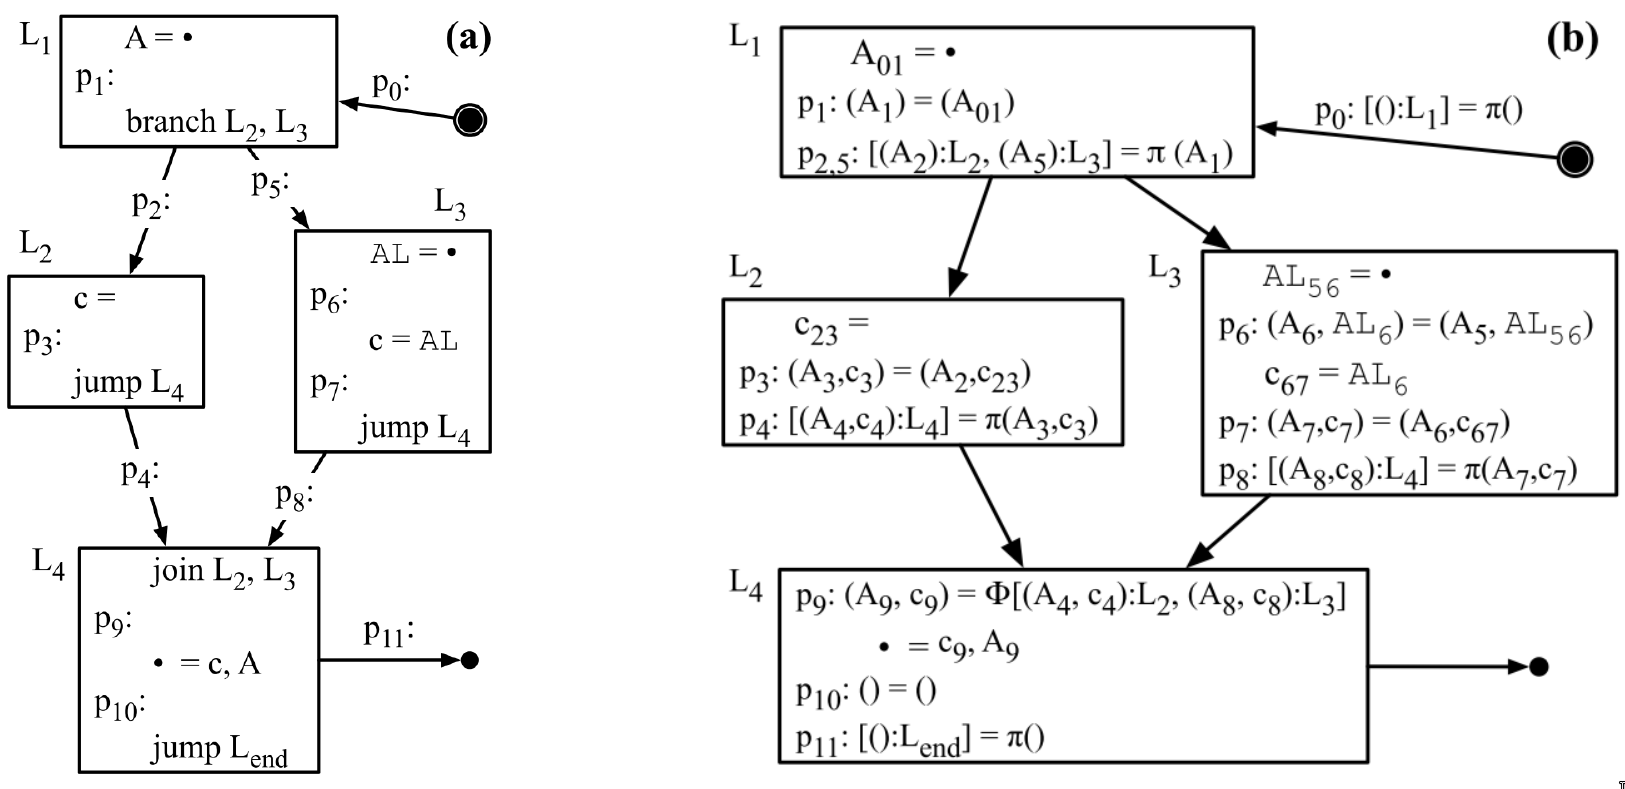
\includegraphics[width=1\linewidth]{figures/elementare-form-example}
\end{center}

\end{frame}

\section{Отображение элементарных программ в фигурки паззлов}

\begin{frame}[fragile]{Виды паззлов}
\noindent{
\begin{minipage}{.66\textwidth}
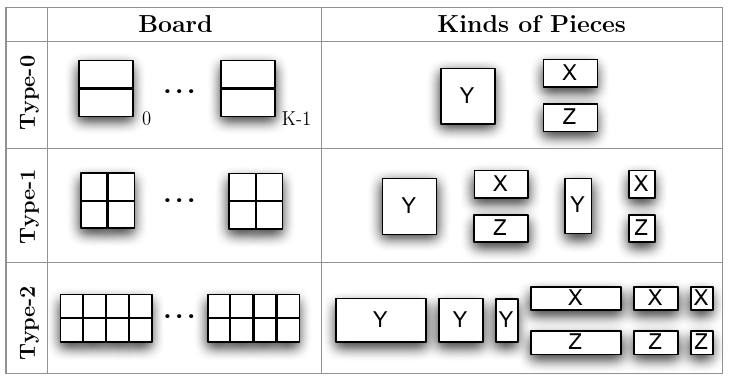
\includegraphics[width=1\linewidth]{figures/puzzle-types}
\end{minipage}}
\begin{minipage}{.32\textwidth}
\begin{itemize}
\item Тип 0: PowerPC \& ARM integers
\item Тип 1: ARM float
\item Тип 2: SPARC V8
\item Гибрид 0+1: x86
\item Гибрид 1+2: SPARC V9
\end{itemize}

\end{minipage}
\end{frame}

%\begin{frame}[fragile]{Add puzzle boards}
%\begin{center}
%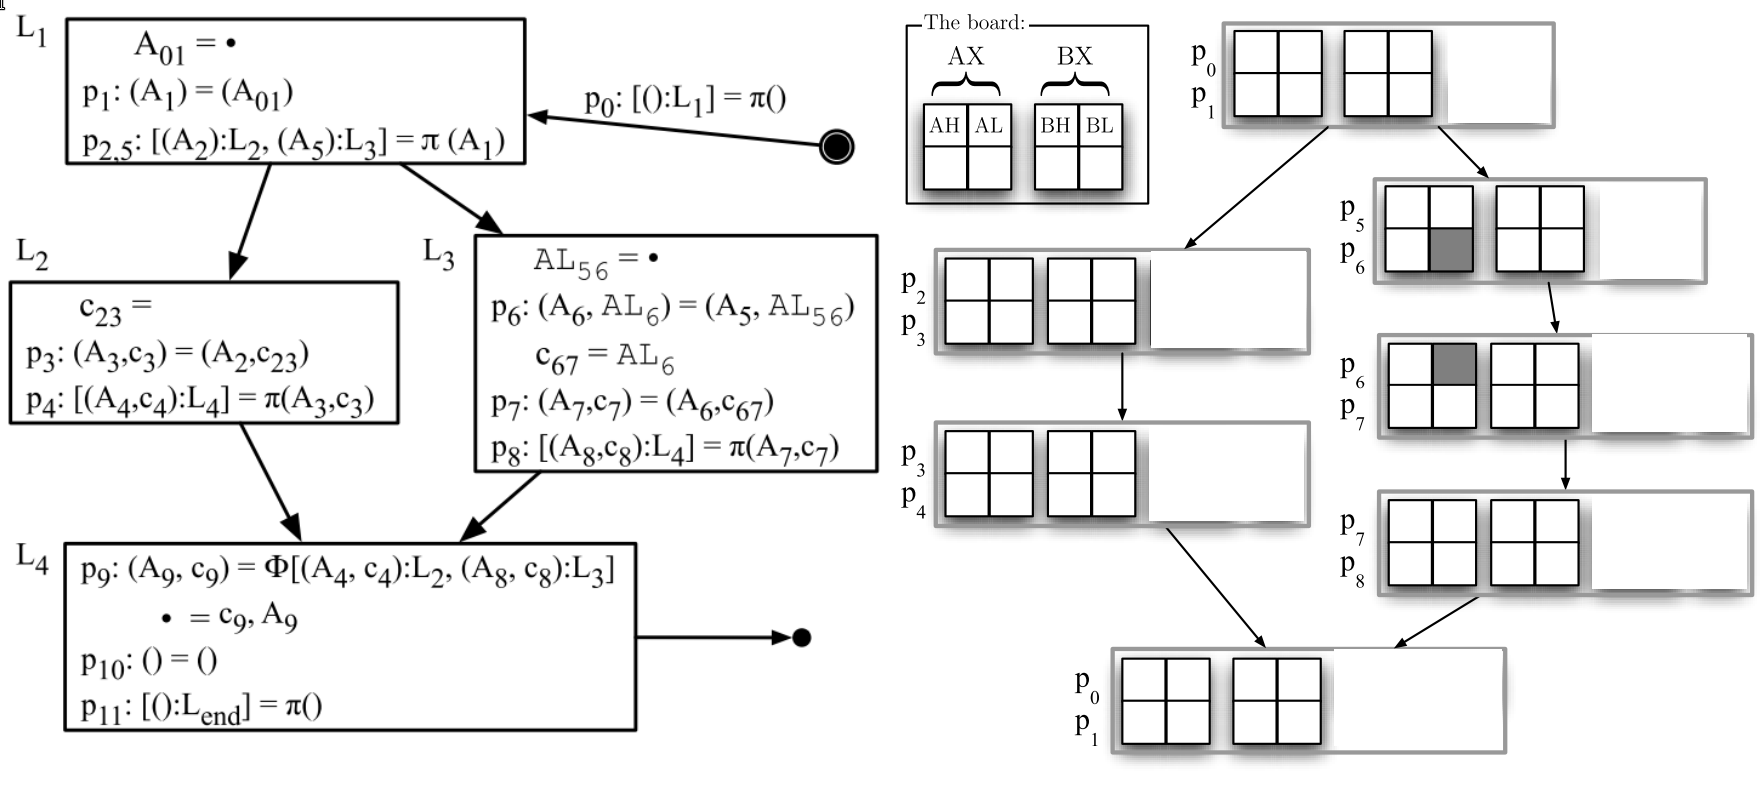
\includegraphics[width=1\linewidth]{figures/add-puzzle-board}
%\end{center}
%
%\end{frame}


\begin{frame}[fragile]{Абстракция паззлов}
\begin{itemize}
\item Паззл = доска (зоны = регистры)  + фигурки (переменные)
\begin{center}
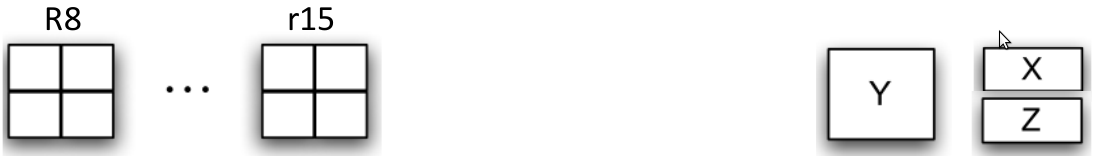
\includegraphics[width=10cm]{figures/puzzle-pieces2.png}
\end{center}
\item  Фигурки не могут перекрываться
\item  Некоторые фигурки могут быть уже выложены на доску
\item  Задача: уместить оставшиеся фигурки на доску (\textbf{register allocation})
\begin{center}
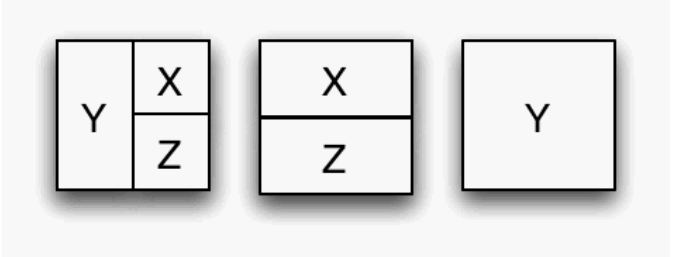
\includegraphics[width=5cm]{figures/puzzle-pieces1.png}
\end{center}
\end{itemize}
\end{frame}


\begin{frame}[fragile]{Создание фигурок паззла}
\noindent{
\begin{minipage}{.65\textwidth}
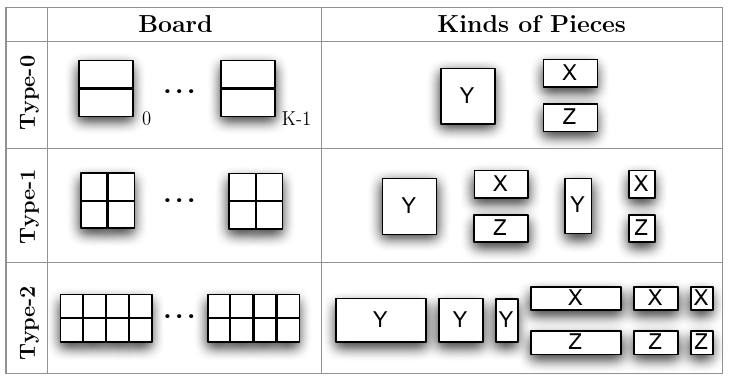
\includegraphics[width=1\linewidth]{figures/puzzle-types}
\end{minipage}}
\begin{minipage}{.33\textwidth}
Для каждой инструкции в программе $i$:
\begin{itemize} 
\item Создать по одной фигурке для live-in и live-out переменных
\item Если переменная перестает быть живой ниже $i$, тогда тип фигурки  X
\item Если переменная начинает быть живой в $i$, тогда Z
\item Иначе Y
\end{itemize}
\end{minipage}
\end{frame}


\begin{frame}[fragile]{Пример. Создание фигурок}
\noindent{
\begin{minipage}{.48\textwidth}
\begin{figure}
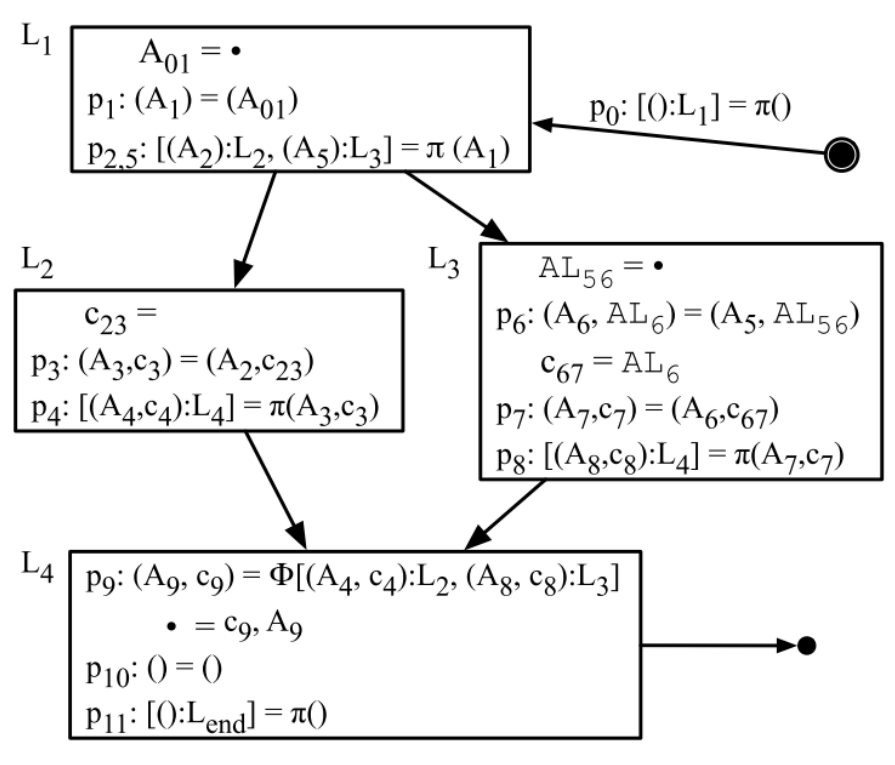
\includegraphics[width=1\linewidth]{figures/someprogram}
\end{figure}
\end{minipage}}
\begin{minipage}{.48\textwidth}
\begin{center}
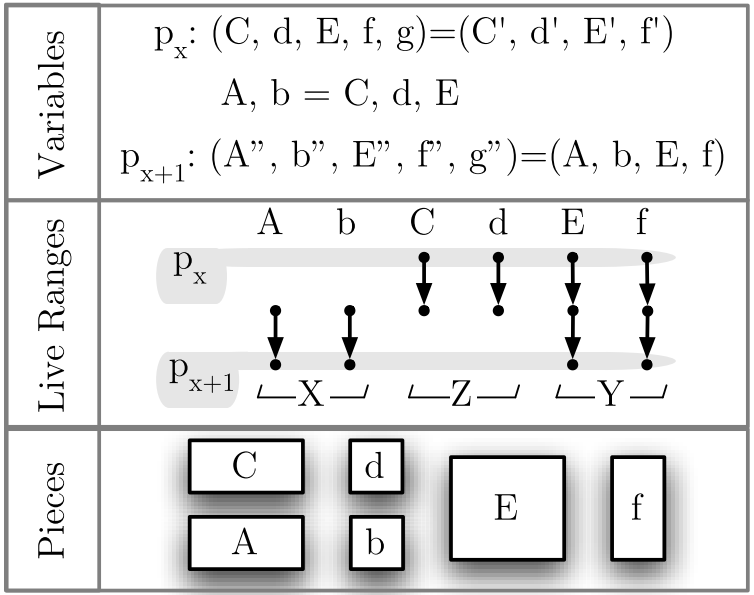
\includegraphics[width=1\linewidth]{figures/creating-pieces}
\end{center}
\end{minipage}
\end{frame}


\begin{frame}[fragile]{Пример. Padding}
\noindent{
\begin{minipage}{.48\textwidth}
\begin{figure}
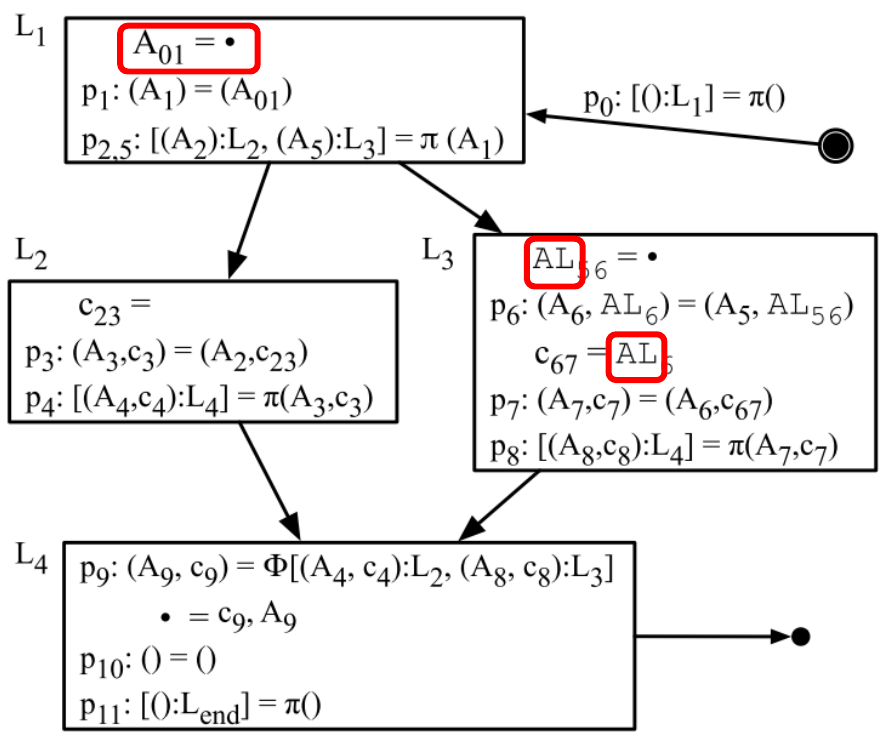
\includegraphics[width=1\linewidth]{figures/someprogram2}
\end{figure}
\end{minipage}}
\begin{minipage}{.48\textwidth}
\begin{center}
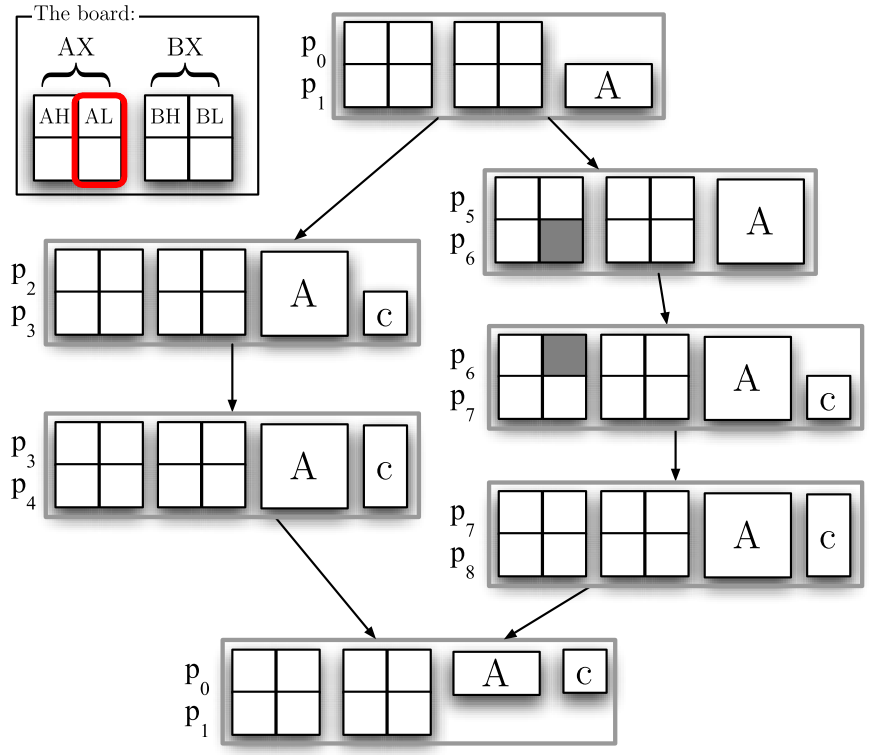
\includegraphics[width=1\linewidth]{figures/dummyname1}
\end{center}
\end{minipage}
\end{frame}


\section{Решаем паззлы}

\begin{frame}[fragile]{Решение паззлов типа 1}
\begin{itemize}
\item Предлагаемый подход: заполнять по одной клетке за раз
\item Ддя каждого квадрата:
  \begin{itemize}
\item Заполняем фигурками X или Z  пока не заполнится вся доска
\end{itemize}
\item Решить задачу
\end{itemize}
\end{frame}


\begin{frame}[fragile]{Решаем паззлы типа 1 визуальным языком (1/3)}
\noindent{
\begin{minipage}{.5\textwidth}
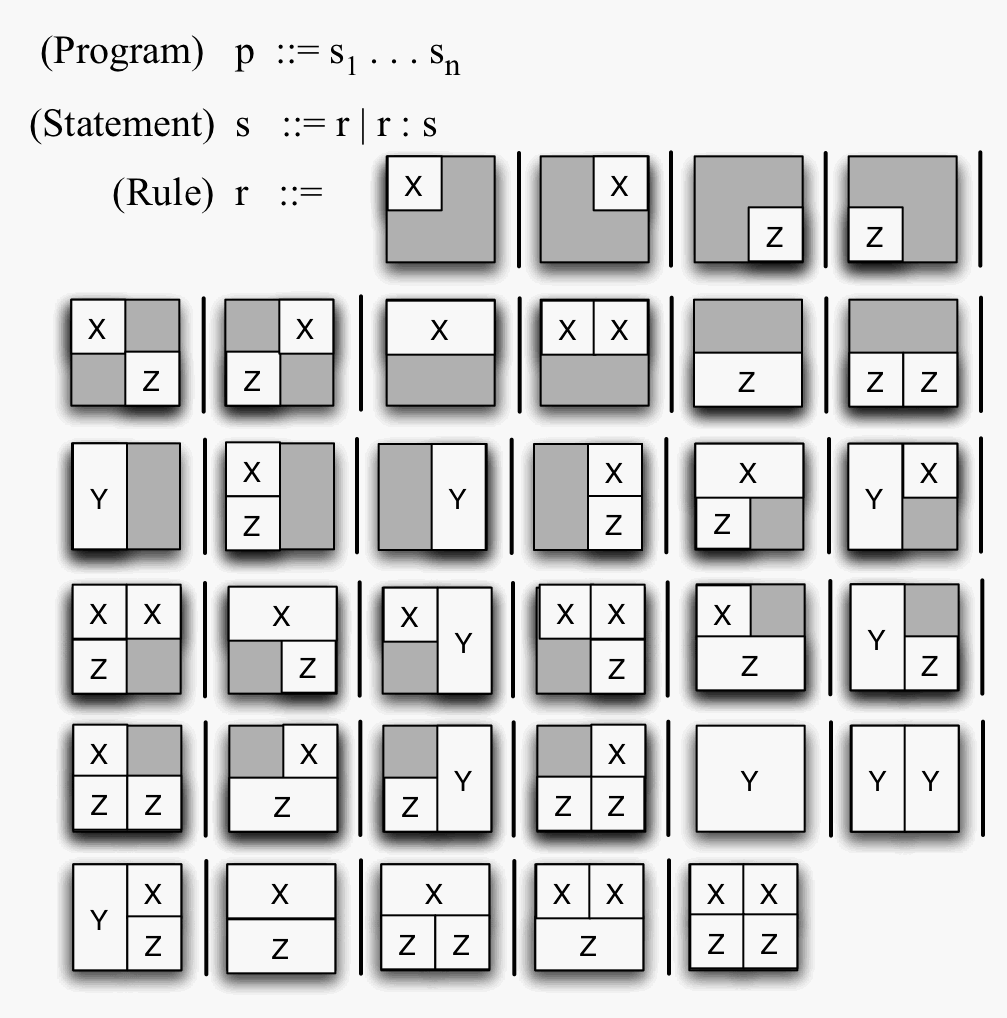
\includegraphics[height=0.85\paperheight]{figures/vis-lang.png}
\end{minipage}}
\begin{minipage}{.48\textwidth}
\begin{itemize}
\item Правило = как заполнять зоны
\item Правилл состоит из
\begin{itemize}
\item шаблона: что уже заполнено (подходит/неподходить под зону)
\item стратегии: какие виды фигурок класть и куда 
\end{itemize}
\item Правило $r$ можно применить на зоне $a$ iff
\begin{itemize}
\item  $r$ подходить к $a$
\item  доступны фигурки для данной стратегии 
\end{itemize}
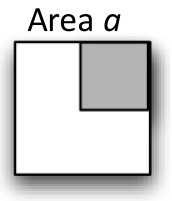
\includegraphics[width=1.5cm]{figures/area-a}
\end{itemize}
\end{minipage}
\end{frame}


\begin{frame}[fragile]{Решаем паззлы типа 1 визуальным языком (2/3)}
\noindent{
\begin{minipage}{.5\textwidth}
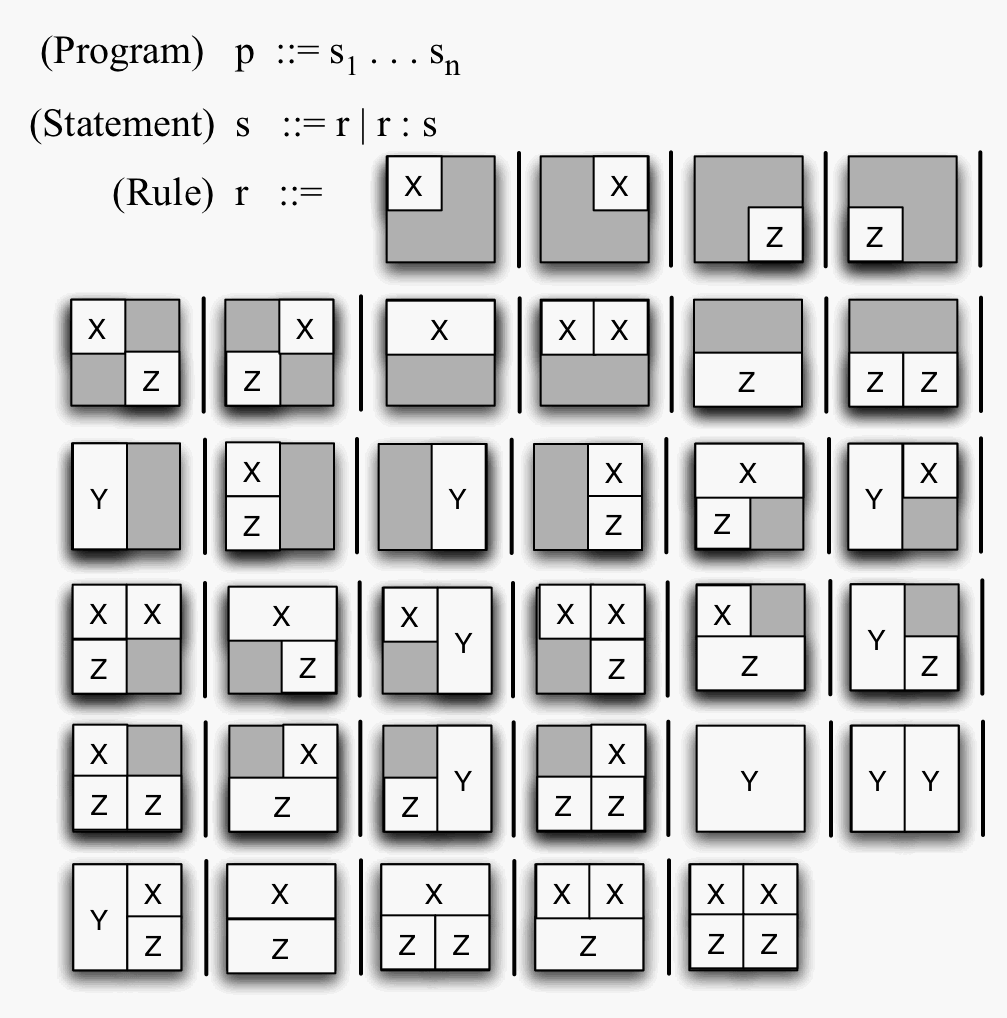
\includegraphics[height=0.85\paperheight]{figures/vis-lang.png}
\end{minipage}}
\begin{minipage}{.48\textwidth}
Условие успешного завершения:
\begin{itemize}
\item Программа успешно завершается iff все утверждения завершаются
\item Правило $r$ можно применить на зоне $a$ iff
\begin{itemize}
\item  $r$ подходить к $a$
\item  доступны фигурки для данной стратегии 
\end{itemize}
\item Условие $(r:s)$ успешно завершается iff
\begin{itemize}
\item r успешно завершается or
\item s успешно завершается
\end{itemize}
\begin{center}
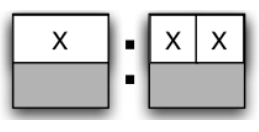
\includegraphics[width=2.5cm]{figures/someurule1}
\end{center}
\end{itemize}
\end{minipage}
\end{frame}

\begin{frame}[fragile]{Решаем паззлы типа 1 визуальным языком (3/3)}
\noindent{
\begin{minipage}{.5\textwidth}
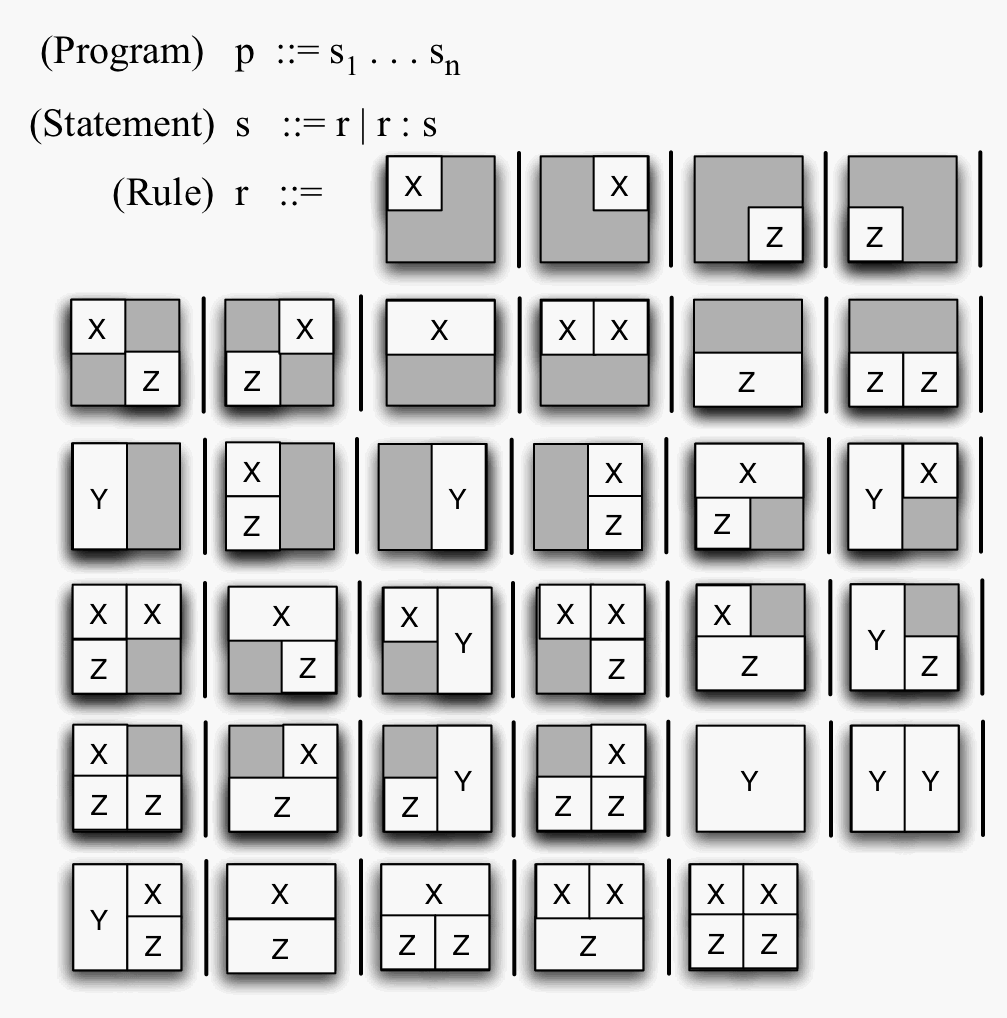
\includegraphics[height=0.85\paperheight]{figures/vis-lang.png}
\end{minipage}}
\begin{minipage}{.48\textwidth}
Исполнение решателя паззлов
\begin{itemize}
\item Для каждой инструкции $s_1, \dots, s_n$
\begin{itemize}
\item Для каждой зоны $a$, такой что паттерн $s_i$ подходит к $a$
\begin{itemize}
\item Применить $s_i$ к $a$
\item Если $s_i$ закончилось и ошибкой, прерваться и сообщить об ошибке
\end{itemize}
\end{itemize}
\end{itemize}
\end{minipage}
\end{frame}



\begin{frame}[fragile]{Исполнение решателя паззлов: пример}
\noindent{
\begin{minipage}{.5\textwidth}
\begin{itemize}
\item Визуальная программа-решатель
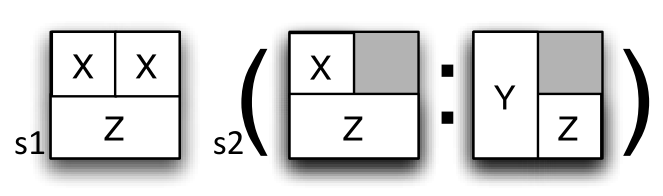
\includegraphics[width=7cm]{figures/puz-example2}
\item Паззл
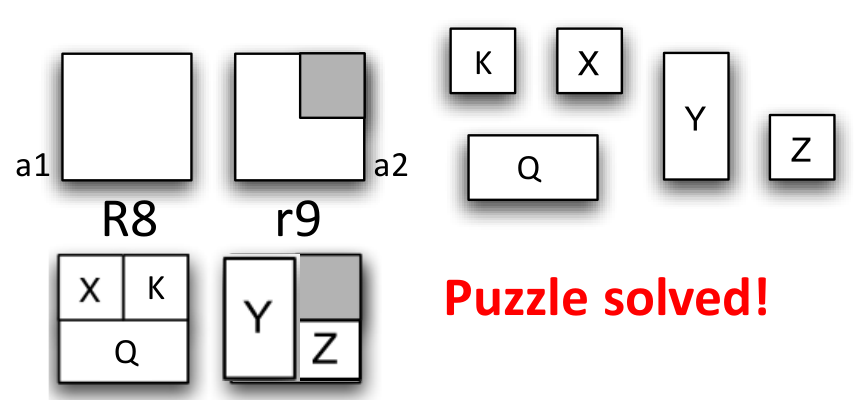
\includegraphics[width=7cm]{figures/puz-example1}
\end{itemize}
\end{minipage}}
\begin{minipage}{.48\textwidth}
\begin{itemize}
\item s1 подходит только к a1 
\item Применение s1 к a1 завершается успешно и выдает результат

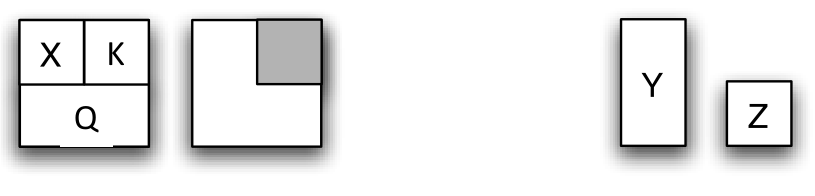
\includegraphics[width=6.5cm]{figures/puz-example3}
\item s2 подходит только к a2
\item Применяем s2 к a2
\begin{itemize}
\item Примение первое правило s2: неудача
\item Применим второе правило s2: успех
\end{itemize}
\end{itemize}
\end{minipage}
\end{frame}

\begin{frame}[fragile]{Исполнение решателя паззлов: другой пример}
\noindent{
\begin{minipage}{.5\textwidth}
\begin{itemize}
\item Визуальная программа-решатель
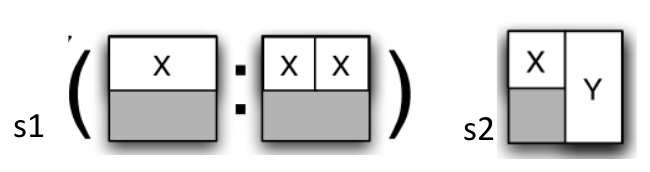
\includegraphics[width=6cm]{figures/puz-example4}
\item Паззл
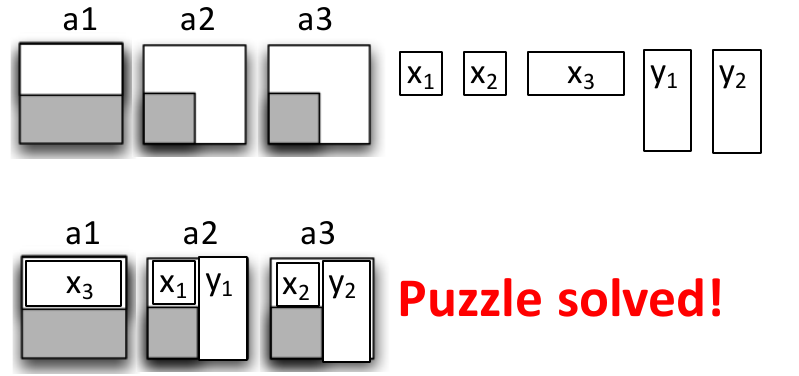
\includegraphics[width=6cm]{figures/puz-example5}
\end{itemize}
\end{minipage}}
\begin{minipage}{.48\textwidth}
\begin{itemize}
\item  s1 подходит только к a1 
\item Применяем s1 к a1 
  \begin{itemize}
  \item  Применяем первое правило к s1: победа
    \begin{center}
    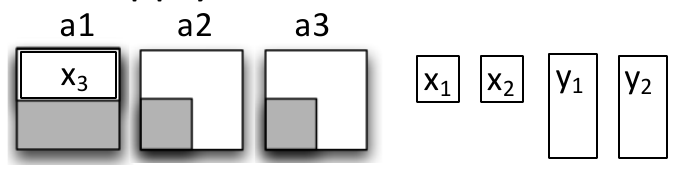
\includegraphics[width=\linewidth]{figures/puz-example6}
    \end{center}  
  \end{itemize}
\item s2 подходит и к  a2, и к a3
\item Применяем s2 к a2

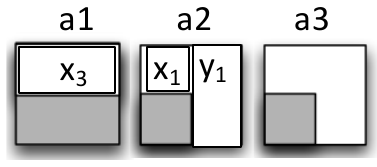
\includegraphics[width=3.5cm]{figures/puz-example7}
\item Применяем s2 к a3
\end{itemize}
\end{minipage}
\end{frame}

\begin{frame}[fragile]{Исполнение решателя паззлов: ещё один пример}
\noindent{
\begin{minipage}{.45\textwidth}
\begin{itemize}
\item Визуальная программа-решатель
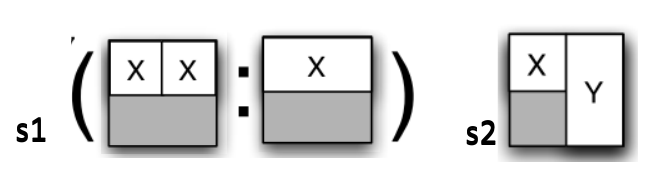
\includegraphics[width=6cm]{figures/puz-example9}

\item Паззл
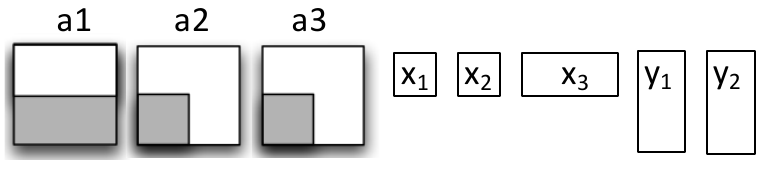
\includegraphics[width=6cm]{figures/puz-example10}
\textcolor{teal}{Построение правильной визуальной программы-решателя существенно!}

\end{itemize}
\end{minipage}}
\begin{minipage}{.53\textwidth}
\begin{itemize}
\item  s1 подходит только к a1 
\item Применяем s1 к a1 
  \begin{itemize}
  \item  Применяем первое правило к s1: победа
    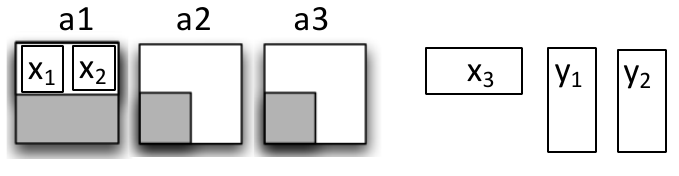
\includegraphics[width=6cm]{figures/puz-example8}
  \end{itemize}
\item s2 подходит и к a2, и к a3
\item Применяем s2 to a2: \textcolor{red}{неудача}\\
Не осталось фигур типа X размера 1: мы использовали их всех
\end{itemize}
\end{minipage}
\end{frame}

\begin{frame}[fragile]{Программа-решатель паззлов типа 1}
\noindent{
\begin{minipage}{.5\textwidth}
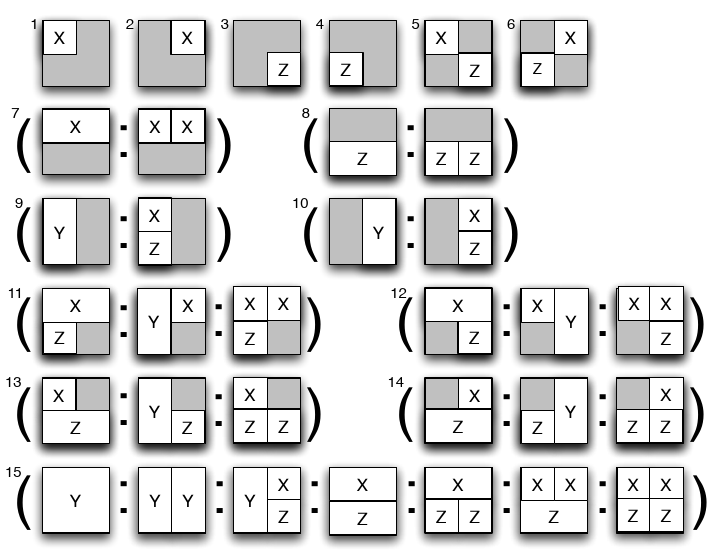
\includegraphics[width=7cm]{figures/type-1-algo}
\end{minipage}}
\begin{minipage}{.48\textwidth}
\begin{theorem}
Задача типа 1 решаема iff эта программа завершается успешно
\end{theorem}

\textcolor{red}{Не решили ли мы  NP задачу за полиномиальное время?}\\


Выделение регистров $\sim$ заполнение всех клеток.\\

Решена более простая задача: заполнение одной клетки за единицу времени
\end{minipage}
\end{frame}



\begin{frame}[fragile]{Решение паззлов типа  1: сложность}
\begin{theorem}
Задача spill-free register allocation (SFRA) с предсраскраской
для элементарной программы $P$ и $K$ регистров решается за $O(\mid\!P\!\mid \times K)$ времени.
\end{theorem}
Для одной инструкции из $P$:
\begin{itemize}
\item Применение правила к зоне: $O(1)$
\item Применяется константное количество правиль к каждой зоне
\item Исполнение на поле с $K$ зонами занимает $O(K)$ времени
\end{itemize}
\end{frame}



\begin{frame}[fragile]{Решаем паззлы  типа 0 (SFRA)}
\noindent{
\begin{minipage}{.6\textwidth}
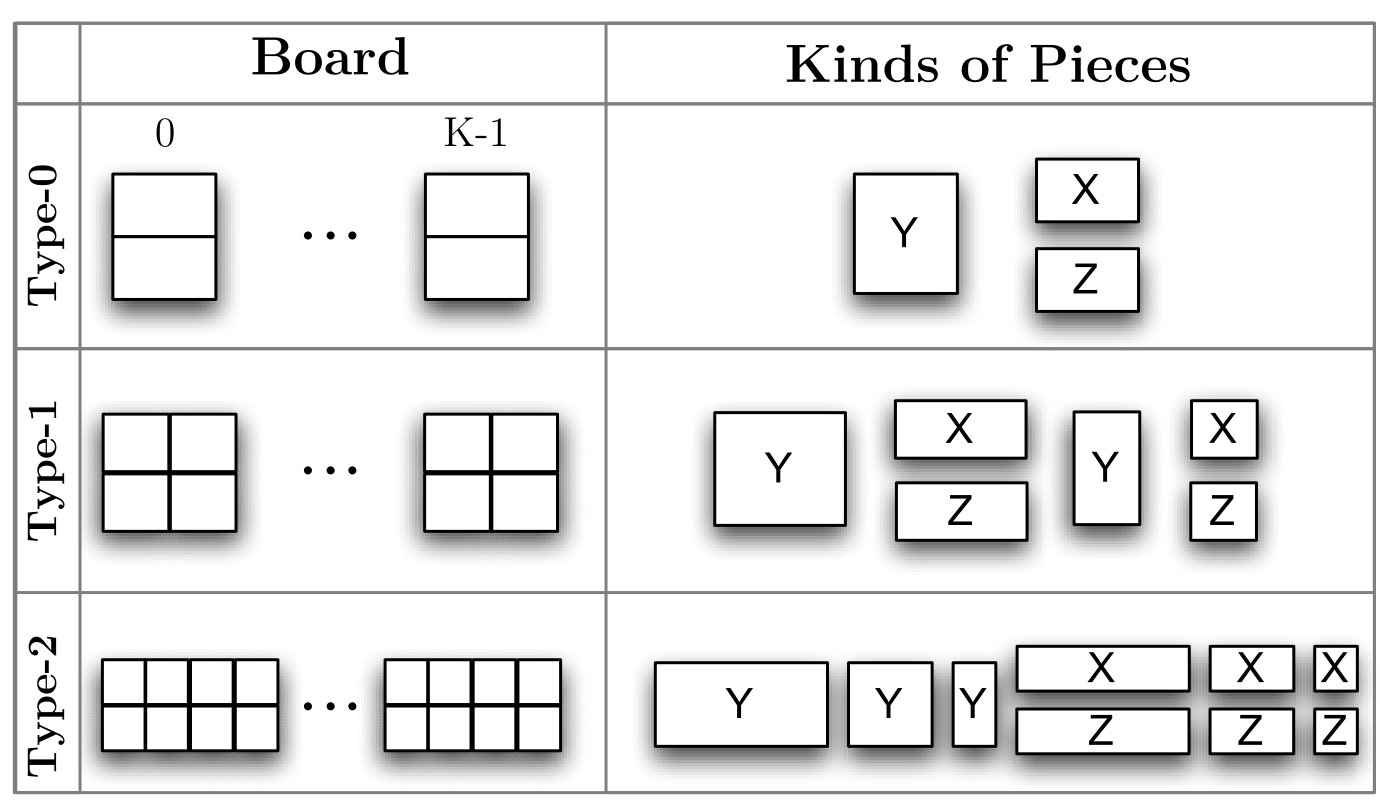
\includegraphics[width=1\linewidth]{figures/puzzles-types}
\end{minipage}}
\begin{minipage}{.38\textwidth}
\begin{itemize}
\item Уложить все Y-фигурки
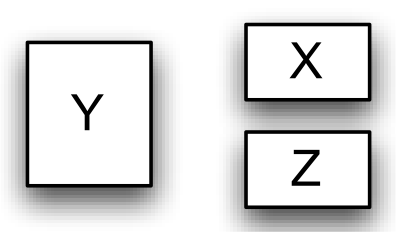
\includegraphics[width=2cm]{figures/puzzles-types-figures}
\item Затем уложить все X и Z фигурки
\end{itemize}
\end{minipage}
\end{frame}


\subsection{Spilling в общем случае}

\begin{frame}{Spilling в общем случае}
\begin{itemize}
\item Если алгоритм для решения SFRA не может решить паззл, (т.е. количество имеющихся регистров не достаточно) => spill
\item Наблюжение: преобразование программы в элементарную форму создаёт семейства переменных для каждой оригинальной переменной % one per original variable
\item Чтобы сделать spill:
\begin{itemize}
\item Выбираем переменную $v$ в оригинальной программе
\item Spillим все переменные из элементарной формы, которые относятся к тому же семейству, что и $v$
\item Для паззлов это будет означать выкидывание фигурок паззла
\end{itemize}
\end{itemize}

\begin{theorem}[Сложность]
Выделение регистров в присутствии предраскрашивания (pre-coloring) и spilling семейства переменных для элементарного представления -- NP-полная задача.
\end{theorem}
\end{frame}



\begin{frame}[fragile]{}
\noindent{
\begin{minipage}{.48\textwidth}
Ещё один метод выделения регистров\\

Генерирует сходный по качеству код, но существенно быстрее, чем использовавшийся до этого в LLVM graph coloring with iterated coalescing.\\
\begin{center}
  {\Huge Конец}\\
\end{center}

\end{minipage}}
\begin{minipage}{.48\textwidth}
\begin{center}
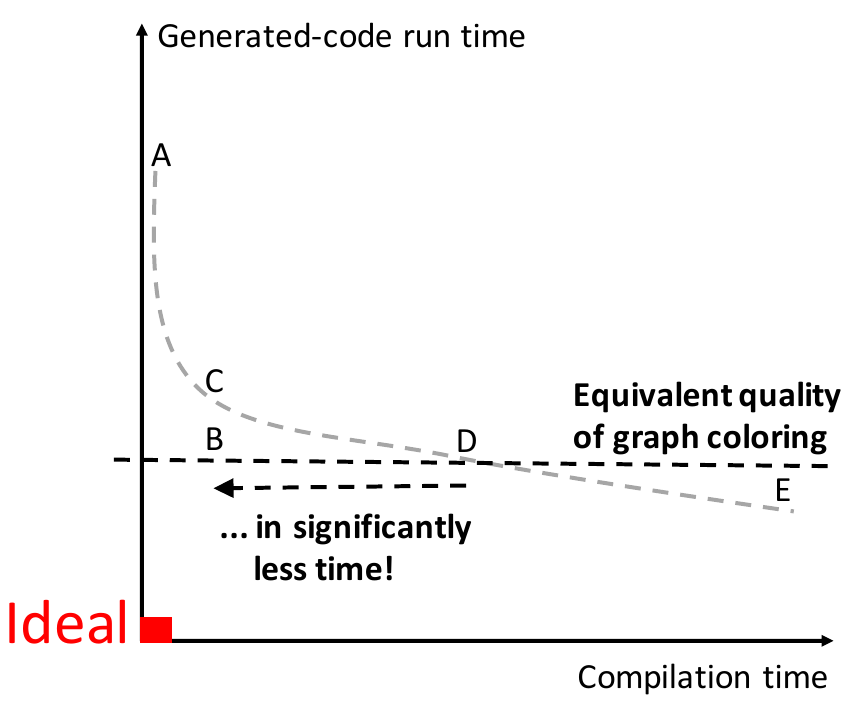
\includegraphics[width=1\linewidth]{figures/all-methods-comparison}
\end{center}

\end{minipage}

\end{frame}



%\begin{frame}[fragile]{}
%\tikzset{every picture/.style={line width=0.75pt}} %set default line width to 0.75pt   
%\begin{tikzpicture}[x=0.75pt,y=0.75pt,yscale=-1,xscale=1]
%%uncomment if require: \path (0,94.5); %set diagram left start at 0, and has height of 94.5
%
%%Shape: Rectangle [id:dp06294366710675758] 
%\draw   (99.76,20) -- (139.65,20) -- (140,40) -- (100.11,40) -- cycle ;
%%Shape: Rectangle [id:dp2425421243241267] 
%\draw   (20,20) -- (60,20) -- (60,60) -- (20,60) -- cycle ;
%%Shape: Rectangle [id:dp944866032756623] 
%\draw   (100,60) -- (139.89,60) -- (140.24,80) -- (100.35,80) -- cycle ;
%
%% Text Node
%\draw (119.88,30) node  [align=left] {X};
%% Text Node
%\draw (120.12,70) node  [align=left] {Z};
%% Text Node
%\draw (40,40) node  [align=left] {Y};
%\end{tikzpicture}
%\end{frame}

%\begin{frame}[fragile]{Контр-пример 1}
%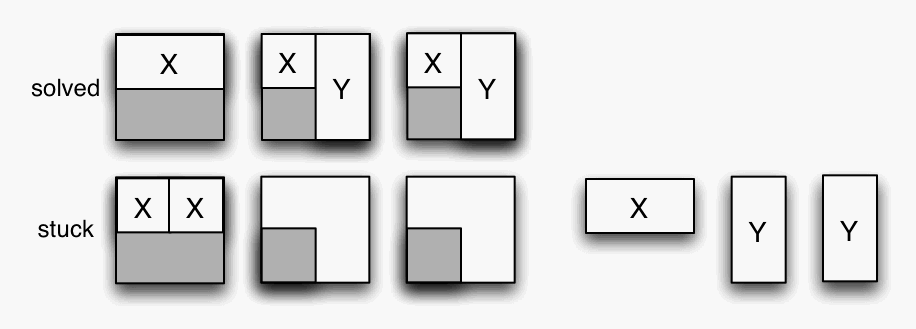
\includegraphics[width=0.9\paperwidth]{figures/ce1.png}
%Lesson: use a size-2 piece before two size-1 pieces
%\end{frame}
%
%\begin{frame}[fragile]{Контр-пример 2}
%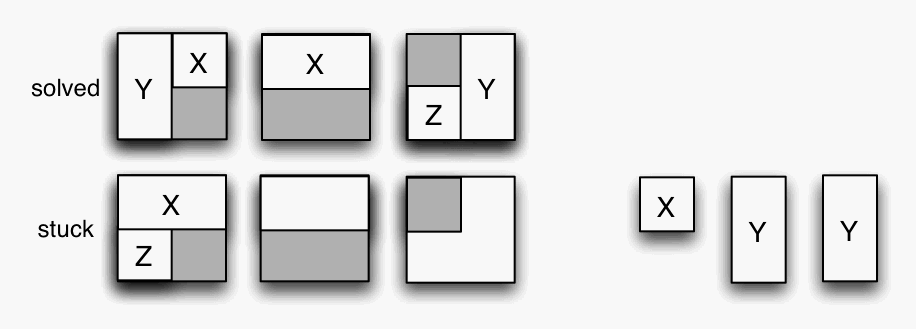
\includegraphics[width=0.9\paperwidth]{figures/ce2.png}
%Lesson: statements 7-10 must come before statements 11-14
%\end{frame}
%
%\begin{frame}[fragile]{Контр-пример 3}
%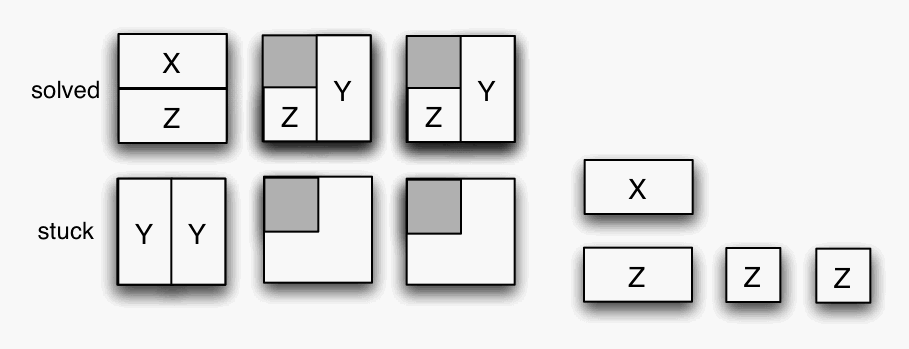
\includegraphics[width=0.9\paperwidth]{figures/ce3.png}
%Lesson: statement 15 must come before statements 11-14
%\end{frame}
%
%\begin{frame}[fragile]{Контр-пример 4}
%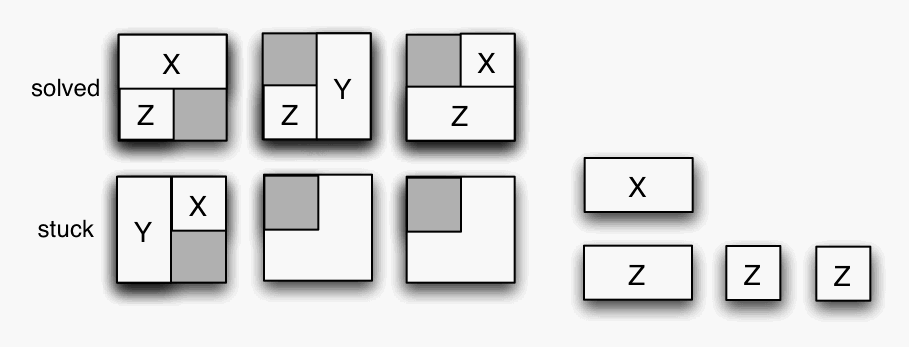
\includegraphics[width=0.9\paperwidth]{figures/ce4.png}
%Lesson: the order in statement 11-14 is crucial
%\end{frame}

%\begin{frame}[fragile]
%\noindent{
%\begin{minipage}{.6\textwidth}
%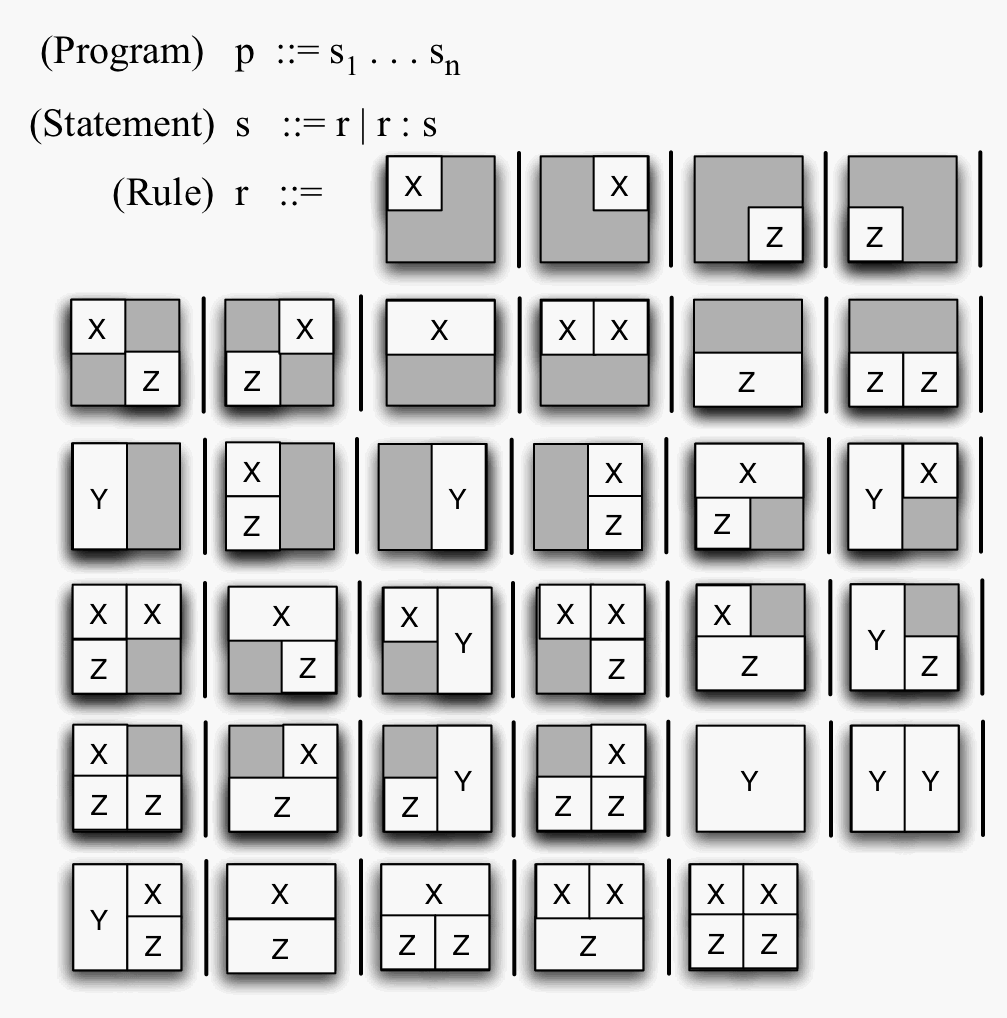
\includegraphics[height=0.9\paperheight]{figures/vis-lang.png}
%\end{minipage}}
%\begin{minipage}{.38\textwidth}
%Визуальный язык для программирования решателей паззлов.
%\end{minipage}
%\end{frame}

%
%
%\begin{frame}
%\begin{center}
%  {\Huge Конец}\\
%  
%\end{center}
%\end{frame}


 \begin{frame}%[allowframebreaks]
   \frametitle<presentation>{Ссылки}
   \begin{thebibliography}{10}
   \bibitem{paper}
     Register Allocation by Puzzle Solving (PLDI 2008)
     \newblock {\em Fernando Magno Quint\~ao Pereira  \& Jens Palsberg }
     \newblock \href{https://llvm.org/pubs/2008-06-PLDI-PuzzleSolving.pdf}{PDF}
           
   \bibitem{thesis}    
     \href{http://compilers.cs.ucla.edu/fernando/publications/papers/PhdDiss.pdf}{PhD thesis}
     \newblock {\em Fernando Magno Quint\~ao Pereira}

   \bibitem{slides1}
     Slides from Compiler Construction course of Northeastern University
     \newblock \href{https://users.cs.northwestern.edu/~robby/courses/322-2016-spring/puzzle_solving.pdf}{PDF}

   \bibitem{ssabook}    
      SSA book
     \href{http://ssabook.gforge.inria.fr/latest/book.pdf}{PDF} 
   \end{thebibliography}
 \end{frame}

\end{document}
